%%%%%%%%%%%%%%%%%%%%%%%%%%%%%%%%%%%%%%%%%
% American Geophysical Union (AGU)
% LaTeX Template
% Version 1.0 (3/6/13)
%
% This template has been downloaded from:
% http://www.LaTeXTemplates.com
%
% Original author:
% The AGUTeX class and agu-ps referencing style were created and are owned
% by AGU: http://publications.agu.org/author-resource-center/author-guide/latex-formatting-toolkit/
%
% This template has been modified from the blank AGU template to include
% examples of how to insert content and drastically change commenting. The
% structural integrity is maintained as in the original blank template.
%
% Important notes:
% This template retains extensive commenting from the AGU template. It is heavily
% advised you read these comments and follow them in order to insure a speedy
% submission process.
%
%%%%%%%%%%%%%%%%%%%%%%%%%%%%%%%%%%%%%%%%%

%%%%%%%%%%%%%%%%%%%%%%%%%%%%%%%%%%%%%%%%%%%%%%%%%%%%%%%%%%%%%%%%%%%%%%%%%%%%
% AGUtmpl.tex: this template file is for articles formatted with LaTeX2e,
% Modified March 2013
%
% This template includes commands and instructions
% given in the order necessary to produce a final output that will
% satisfy AGU requirements.
%
% PLEASE DO NOT USE YOUR OWN MACROS
% DO NOT USE \newcommand, \renewcommand, or \def.
%
% FOR FIGURES, DO NOT USE \psfrag or \subfigure.
%
%%%%%%%%%%%%%%%%%%%%%%%%%%%%%%%%%%%%%%%%%%%%%%%%%%%%%%%%%%%%%%%%%%%%%%%%%%%%
%
% All questions should be e-mailed to latex@agu.org.
%
%%%%%%%%%%%%%%%%%%%%%%%%%%%%%%%%%%%%%%%%%%%%%%%%%%%%%%%%%%%%%%%%%%%%%%%%%%%%

% Step 1: Set the \documentclass

% There are two options for article format: two column (default) and draft.

% PLEASE USE THE DRAFT OPTION TO SUBMIT YOUR PAPERS.
% The draft option produces double spaced output.

% Choose the journal abbreviation for the journal you are submitting to:

% jgrga	JOURNAL OF GEOPHYSICAL RESEARCH
% gbc	GLOBAL BIOCHEMICAL CYCLES
% grl		GEOPHYSICAL RESEARCH LETTERS
% pal	PALEOCEANOGRAPHY
% ras	RADIO SCIENCE
% rog	REVIEWS OF GEOPHYSICS
% tec	TECTONICS
% wrr	WATER RESOURCES RESEARCH
% gc		GEOCHEMISTRY, GEOPHYSICS, GEOSYSTEMS
% sw	SPACE WEATHER
% ms	JAMES
%
%
%
% (If you are submitting to a journal other than jgrga,
% substitute the initials of the journal for "jgrga" below.)

\documentclass[draft, jgrga]{AGUTeX}

% can I use these symbols?
\usepackage{array,amssymb}

% permil symbol
\usepackage{ wasysym }

% To create numbered lines:

% If you don't already have lineno.sty, you can download it from http://www.ctan.org/tex-archive/macros/latex/contrib/ednotes/ (or search the internet for lineno.sty ctan), available at TeX Archive Network (CTAN). Take care that you always use the latest version.

% To activate the commands, uncomment \usepackage{lineno} and \linenumbers*[1]command, below:

%\usepackage{lineno}
%\linenumbers*[1]

%  To add line numbers to lines with equations:
%  \begin{linenomath*}
%  \begin{equation}
%  \end{equation}
%  \end{linenomath*}

%%%%%%%%%%%%%%%%%%%%%%%%%%%%%%%%%%%%%%%%%%%%%%%%%%%%%%%%%%%%%%%%%%%%%%%%%
% Figures and Tables

% DO NOT USE \psfrag or \subfigure commands.

%  Figures and tables should be placed AT THE END OF THE ARTICLE, after the references.

%  Uncomment the following command to include .eps files (comment out this line for draft format):
%\usepackage[dvips]{graphicx}
\usepackage{graphicx}
\usepackage{caption}
%\usepackage{subfig}


% Substitute one of the following for [dvips] above if you are using a different driver program and want to proof your illustrations on your machine:
% [xdvi], [dvipdf], [dvipsone], [dviwindo], [emtex], [dviwin],
% [pctexps],  [pctexwin],  [pctexhp],  [pctex32], [truetex], [tcidvi],
% [oztex], [textures]

%  Uncomment the following command to allow illustrations to print when using Draft:
\setkeys{Gin}{draft=false}

% See how to enter figures and tables at the end of the article, after references.

%----------------------------------------------------------------------------------------
%	RUNNING HEAD AND CORRESPONDING AUTHOR
%----------------------------------------------------------------------------------------

% Author names in capital letters:
\authorrunninghead{Authors}

%------------------------------------------------

% Shorter version of title entered in capital letters:
\titlerunninghead{CFA DATA DIFFUSION LENGTHS}

%------------------------------------------------

% Corresponding author mailing address and e-mail address:
\authoraddr{Corresponding author: Emma Kahle, Earth and Space Sciences Department, University of Washington, Seattle, WA, USA. (eckahle@uw.edu)}

%----------------------------------------------------------------------------------------

\begin{document}

%----------------------------------------------------------------------------------------
%	TITLE
%----------------------------------------------------------------------------------------

\title{Estimating diffusion lengths of water isotopes from ice core data measured by continuous flow analysis}

%----------------------------------------------------------------------------------------
%	AUTHORS AND AFFILIATIONS
%----------------------------------------------------------------------------------------

% Use \author{\altaffilmark{}} and \altaffiltext{}

% \altaffilmark will produce footnote; matching \altaffiltext will appear at bottom of page.

\authors{Emma Kahle,\altaffilmark{1}
Christian Holme,\altaffilmark{2}, and
everyone else}

\altaffiltext{1}{Department of Earth and Space Sciences, University of Washington, Seattle, Washington, USA.}

\altaffiltext{2}{The Niels Bohr Institute, Centre for Ice and Climate, Juliane Maries Vej 30, 2100 Copenhagen, Denmark}

%----------------------------------------------------------------------------------------
%	ABSTRACT
%----------------------------------------------------------------------------------------

% Do NOT include any \begin...\end commands within the body of the abstract.

\begin{abstract}

We examine high-resolution water isotope data sets from continuous flow analysis (CFA) of the West Antarctic Ice Sheet (WAIS) Divide (WDC) and South Pole (SPC) ice cores. Spectral analysis of water isotope data reveals damping of high-frequency variations associated with diffusive smoothing of the isotopic profile in the firn layer of an ice sheet. This diffusion of water isotope ratios in ice cores can provide information about past firn conditions. The spectra of windowed sections of CFA data from WDC and SPC show different characteristics than those from discretely-sampled data sets due to their higher resolution and greater signal to noise ratio. This difference affects the estimation of high-frequency damping due to the firn diffusion process, and previous techniques are unable to capture the extent of diffusion on these CFA data sets. We propose two estimation techniques that apply generally to both CFA and discretely-sampled data in order to efficiently and accurately produce diffusion estimates for all ice core data sets. We demonstrate the application of these results to estimate temperature change and investigate firn processes through time.

\end{abstract}

%----------------------------------------------------------------------------------------
%	ARTICLE CONTENT
%----------------------------------------------------------------------------------------

% The body of the article must start with a \begin{article} command
% \end{article} must follow the references section, before the figures and tables.

\begin{article}

\section{Introduction}

To understand past and future climate change, water isotope data from ice cores have long been used as climate proxies, based on the temperature-dependent distillation of water isotope ratios (e.g. $\delta^{18}\mathrm{O}$) in the atmosphere (\citep{Epstein1951,Dansgaard1954,Dansgaard1964}). This indirect method for obtaining temperature records through past glacial and interglacial cycles relies on empirical correlations that only approximate the physical processes involved. A more direct approach uses the signal of isotope diffusion preserved in the ice, overcoming the many issues related to the conventional
isotope method \citep{Johnsen2000}.

\subsection{Stable Water Isotope Diffusion}

Water isotope diffusion occurs primarily in the firn layer, snowfall in the upper tens of meters of an ice sheet that has yet to be fully compressed into ice. Because firn is permeable, water molecules can diffuse through in the vapor phase, damping the seasonal variations and high-frequency noise of the original isotope signal. As the diffusion process depends on temperature, a temperature record can be obtained by measuring the extent of diffusion that has occurred \citep{Johnsen2000}. This method is independent of conventional assumptions about isotope fractionation before deposition, and thus improves on conventional ice core temperature methods. Beyond information about past temperature, diffusion estimates also provide constraints on past firn conditions and total ice thinning. With these motivations, estimations of diffusion have been made for ice cores in both Greenland and Antarctica \citep{Simonsen2011,Gkinis2014,vanderWel2015,Jones2017a}. Past studies have outlined the math behind this theory, and we thoroughly derive these equations in Appendices A through D.

\subsection{Measurement of Ice Core Water Isotopes}

In the past, most ice core water isotope data have been measured discretely by melting vertical sections of the core to produce a sample. The isotope ratio of each discrete sample is measured by mass spectrometry or laser spectroscopy (cite papers). Recently, ice core water isotope measurements are often measured on continuous flow analysis (CFA) systems. These systems continuously feed the water stable isotopes of the melting core directly into a laser spectrometer, yielding high resolution data more easily \citep{Gkinis2011a,Emanuelsson2015,Jones2017b}. Depending on the amount of effort committed, discrete analyses can produce resolutions ranging from one-meter for entire ice cores to $\sim$1-cm for smaller sections of ice cores. Meanwhile, CFA analyses can easily produce results at half-cm resolution for an entire ice core record. This higher resolution has the potential to improve the ability to analyze diffusion lengths, which depend on information in the high frequencies of the data spectrum.

\subsection{Water Isotope Data}

We use data from the WAIS Divide (WDC) \citep{Jones2017b} and South Pole (SPC) \citep{Casey2014} ice cores, both measured continuously at the Institute of Arctic and Alpine Research (INSTAAR) at the University of Colorado. We use the first 2800 meters of WDC, corresponding to approximately 30,000 years. As of this writing, the full SPC record is still being analyzed, but we use two 50-meter sections, one from the Holocene and one from the last glacial period. INSTAAR uses a CFA system to measure the water isotope ratios of $\delta^{18}\mathrm{O}$, $\delta^{17}\mathrm{O}$, and $\delta\mathrm{D}$ at a resolution of half-cm. The CFA system was developed throughout the measurement of WDC, and the same methods were used to measure SPC. For complete details on the INSTAAR CFA system, see \citet{Jones2017b}. For comparison we use other published discrete and continuous water isotope data sets from Greenland and Antarctic cores presented in \citet{Oerter2004,Gkinis2011a,Steig2013,Svensson2015,Holme2017}.

The spectra of these CFA data have different characteristics than discretely-sampled data due to their higher resolution and greater signal to noise ratio. Discretely-sampled data have been effectively analyzed for diffusion lengths by a number of studies \citep{Johnsen2000,Simonsen2011,Gkinis2014,vanderWel2015} and match well with spectra from theoretically derived synthetic data \citep{Holme2017}. However, these diffusion estimation methods can not be applied to spectra from CFA data due to an additional characteristic in the mid-frequency range ($10-40$ cycles/m $\approx 2.5-10$ cm ice) exposed by the lower baseline noise level. Figure \ref{spectra_disVScfa} demonstrates this spectral difference by comparing the spectra of discretely- and continuously-measured data. The CFA spectra have a ``transition zone" where power decreases approximately linearly from the diffusion-damped frequencies into the higher-frequency noise of the measurement system. The highest-resolution discretely-sampled data sets do not show this transition zone in the spectrum.

Because estimating diffusion length depends on the shape of the spectrum, the presence of this transition zone affects calculation of diffusion length using conventional methods. In this paper we describe how to estimate diffusion lengths on CFA data despite the existence of this transition. We start with the approaches developed in \citet{Johnsen2000} and \citet{Gkinis2014} and propose two adjusted techniques to accommodate this transition in CFA water isotope data.

%------------------------------------------------

\section{Diffusion Theory}

The fundamental physics of advection and diffusion can describe mathematically the post-depositional effects on the profile of water isotopes in the ice core \citep{Johnsen1977}. The majority of water isotope diffusion occurs in the firn layer where interconnected air pathways allow water vapor to diffuse vertically through the firn column. After firn densification has sealed off bubbles in the ice, vapor diffusion ceases and solid ice diffusion takes over. The process in solid ice has a diffusivity orders of magnitude smaller than that of vapor diffusion, and we do not consider it in this study.

The isotopic profile changes through the firn layer of an ice sheet due to the effects of diffusion across isotopic gradients and due to densification of the firn. As shown by \citet{Johnsen1977} and subsequently used in several diffusion studies (\citep{Johnsen2000, Simonsen2011, Gkinis2014, vanderWel2015, Jones2017a, Holme2017}), these changes to the isotopic profile can be described by Fick's second law, the basic advection-diffusion equation:
\begin{equation}
\frac{\partial \delta}{\partial t}
= D \frac{\partial ^2 \delta}{\partial z^2}
- \dot{\epsilon}
z \frac{\partial \delta}{\partial z}
\end{equation}

\noindent where \begin{math} \delta \end{math} is the isotope ratio, \begin{math} D \end{math} is the diffusivity coefficient, \begin{math} z \end{math} is the vertical coordinate assuming an origin fixed on a sinking layer of firn, and \begin{math} \dot{\epsilon} \end{math} is the vertical strain rate. The term \begin{math} \dot{\epsilon} z \end{math} can be thought of as the vertical velocity in this advection-diffusion framework. Considering a layer of firn with \begin{math} z = 0 \end{math} at the vertical midpoint, \begin{math} \dot{\epsilon} z \end{math} is the rate at which a point distance \begin{math} z \end{math} from \begin{math} z=0 \end{math} approaches the origin. A solution for the isotopic profile at time $t$ and at depth $z$ in the firn column is given by:
\begin{equation}
\label{eq:diff_sol}
\delta (z,t) = S(t) \frac{1}{\sigma \sqrt{2 \pi}}
\int^\infty_{-\infty} \delta (z,0) \exp \left(\frac{-(z-u)^2}{2 \sigma ^2} \right)du
\end{equation}

\noindent where \begin{math} S(t) \end{math} is the total thinning the layer has experienced due to ice flow from $t=0$ to $t=t'$:
\begin{equation}
S(t') = exp \left( \int^{t'}_{0} \dot{\epsilon}(t) dt \right)
\end{equation}

Previous studies layout these main equations, but many of the derivation details are left out. For detailed analytical and statistical derivations of the solution in Equation \ref{eq:diff_sol}, see Appendices A and B.

The amount of smoothing applied to the signal in Equation \ref{eq:diff_sol} can be quantified as a diffusion length, or the average vertical distance traveled by a water molecule before it reaches the bottom of the firn. Appendix C gives a statistical derivation of diffusion length, an intuitive explanation of the definition of diffusion length.

%------------------------------------------------

\section{Estimating Diffusion Length from Data (methods)}
\subsection{Basic/Theoretical/Conventional Approach}

With a mathematical understanding of water isotope diffusion, we can match diffusion lengths calculated from ice core data to modeled diffusion lengths to learn about past firn conditions, including temperature, densification, and ice thinning. To make this comparison, we require a method to estimate diffusion lengths from the ice core data. Equation \ref{eq:diff_sol} demonstrates that the ice core data, $\delta(z,t)$, is the convolution of the initial isotope signal $\delta(z,0)$ with a Gaussian filter of standard deviation of the diffusion length $\sigma$ \citep{Johnsen2000}:
\begin{equation}
\mathcal{G} = \frac{1}{\sigma \sqrt{2\pi}} \exp \left( \frac{-z^2}{2\sigma^2} \right)
\end{equation}

To solve this convolution, we take the Fourier transform of both sides of the equation:
\begin{equation}
  \delta(z,t) = \delta(z,0)*\mathcal{G} \qquad \Rightarrow \qquad \hat{\delta}(z,t) = \hat{\delta}(z,0)\hat{\mathcal{G}}
\end{equation}

where $*$ represents the convolution and \quad $\hat{}$ \quad represents the Fourier transform. The Fourier transform of a Gaussian remains a Gaussian:
\begin{equation}
\mathfrak{F}(\mathcal{G}) = \hat{\mathcal{G}} = \exp \left( \frac{-k^2\sigma^2}{2} \right)
\end{equation}

where $k$ is wavenumber.

With the assumption that the initial isotope signal $\delta(z,0)$ can be approximated as white noise \citep{Gkinis2014}, we can fit, in frequency space, a Gaussian curve to the data spectrum and solve for its standard deviation. The standard deviation $\varsigma$ of the frequency-space Gaussian is related to the diffusion length $\sigma$ by:
\begin{equation}
  \sigma = \frac{1}{2\pi\sqrt{2}\varsigma}
\end{equation}

Appendix D derives this conversion factor, explaining how a Gaussian fit in the frequency domain can be converted into a diffusion length in the depth domain. Repeating this method over consecutive windowed sections of data yields diffusion length estimates through the length of a core.

Fitting the data spectrum is complicated when working with CFA data (refer back to Figure \ref{spectra_disVScfa}). \citet{Jones2017a} avoids the effect of the CFA transition zone by identifying the frequency at which the transition intersects the damping of diffusion. The technique cuts off frequencies above this intersection, and includes only lower frequencies in the Gaussian fit. Figure \ref{cutoff} shows examples of this cut-off technique for data sections from WDC and SPC. This technique relies on the fact that the cut-off frequency at the intersection of the transition zone preserves enough of the signal to make a good Gaussian fit.

\subsection{New Approach}
In this study we start with the fitting approach of \citet{Gkinis2014} for discrete data, which uses a least-squares technique to fit the sum of two functions ($P_s$) to the spectra of ice core data by varying the four parameters $P_0$, $\sigma^2$, $a_1$ and $\varsigma_{\mathrm{\eta}}^2$:

\begin{equation}
P_s =    P_0 {e}^{-k^2 \sigma^2} + \frac{\varsigma_{\mathrm{\eta}}^2 \Delta}
{\left| 1-a_1 \exp{\left( -i k  \Delta \right) } \right|^2},
\label{eq:powerspectrum}
\end{equation}

\noindent where $a_1$ is the AR-1 coefficient, $\varsigma_{\mathrm{\eta}}^2$ is the variance of the noise signal and $\frac{1}{\Delta}$ is the sampling frequency. The first function is a Gaussian, representing the high-frequency damping of firn diffusion, and the second function is an autoregressive noise signal of order 1 (AR-1), representing baseline noise introduced by measurement and post-depositional processes. Adding together these two functions avoids having to choose a cut-off frequency for the fit. Since it does not require any subjective choices, this two-function technique can be fully automated and produce results in less time and with less effort than the cut-off technique.

This two-function technique has been used effectively to estimate diffusion lengths on many discretely sampled data sets \citep{Gkinis2014,Holme2017}. When applying this technique to CFA data sets, the transition zone in the CFA spectra affects the technique's ability to effectively fit a Gaussian to the data. Figure \ref{GR_fits} illustrates this issue with examples of WDC and SPC spectra. The presence of the transition zone forces both the Gaussian and noise functions to accommodate its shape. The standard deviation of the Gaussian function increases, corresponding to a smaller diffusion length, and the noise level increases slightly at lower frequencies. The poor total fit of the data results in a poor representation of diffusion length.

\section{Generalizing the fitting technique}
To generalize the fitting technique to function for CFA data as well as discrete data, we consider two different approaches. The first approach removes the transition zone by masking it with white noise, allowing the spectra to be fit effectively by two functions, as above. The second approach builds on the two-function technique by including an extra function in the parameterization. In this section, each technique is introduced and illustrated on spectra from WDC and SPC.

\subsection{Technique 1: Adding white noise}
The main differences between CFA data and discrete data are the resolution and precision. These differences result in the presence of the transition zone due to a lower white noise baseline for the high frequencies in the CFA data compared to the measurement baseline of the discrete data, as shown in Figure \ref{spectra_disVScfa}. In order to fit the CFA spectrum, this technique masks the transition zone in the CFA data. We add Gaussian-distributed noise in the time domain, which increases the white-noise level in the frequency domain. The transition zone is hidden under this added noise, and the resulting power spectrum is similar to that of older, less-precise CFA and discrete measurements. The two-function technique of \citet{Gkinis2014} can now be effectively applied to the spectrum. The disadvantage of this technique is that it manipulates the orginal signal; while the added noise masks the transition zone, it may also mask useful climate information. Figure \ref{WAIS_spectrum_added_noise} illustrates this technique with a WDC spectrum.

We used a sensitivity test to quantify the best choice of added noise level. The test uses a 500-year moving window throughout the WDC record. For each windowed section, 100 diffusion lengths are estimated by adding an increasing white noise baseline to the data in each window. A diffusion length is estimated for each tested noise level on each 500-year window. Adding too little noise does not effectively mask the transition zone, but adding too much noise risks masking the climate signal. We define the optimal noise level as that with which the diffusion length estimates stop changing with increasing noise. This level can be found when the gradient of diffusion length with respect to added noise level approaches zero. Fig \ref{added_noise_sensitivity} shows this how this gradient changes for both $\delta^{18}$O and $\delta$D throughout the WDC core. For WDC, the optimal added noise for $\delta^{18}$O is Gaussian-distributed noise with a standard deviation of $0.4 \, \permil$ and for $\delta$D is a standard deviation of $3.0 \,\permil$.

\subsection{Technique 2: Parameterizing a multi-function fit}
The second approach creates a multi-function parameterization of the total spectrum by adding a third function to the Gaussian and noise functions of the two-function technique. We test three different functions to determine which addition yields the best full-spectrum fit. First, we add a second AR-1 function; second, we add a second Gaussian curve; third, we add a folded normal distribution (FND) \citep{Tsagris2014}:
\begin{equation}
P_{FND} = P_{0_{FND}} \cdot e^{-(k \cdot \sigma_{FND})^2} \cdot |\left[1 - \Phi(-i k \sigma_{FND})\right]|^2,
\end{equation}
where $\Phi(\sigma_{FND}) = 1/2\cdot \mathrm{erfc}(-\sigma_{FND}/2) $. Here $P_0$ and $\sigma_{FND}$ are the two parameters that are varied to optimize the fit. The justification of fitting a FND is that it reflects the unidirectional memory and diffusion induced by the one-way flow of the CFA system. A FND is the absolute value of a Gaussian distribution, resulting in a function that smooths in only one direction. Because water is continuously flowing in one direction in the CFA system, the application of a FND mimics this one-sided effect. Thus if this unidirectional effect of the CFA system is significant, we expect the FND function to fit the data well.

The results of each of these three parameterizations for WDC and SPC are shown in Figures \ref{GRR_fits} through \ref{folded_normal_gauss_spectrum}. Figure \ref{GRR_fits} shows the first parameterization, which sums a Gaussian curve and two autoregressive noise functions. With the inclusion of this third function in both WDC and SPC, the total fit is visually improved, as compared to the single-Gaussian fit in Figure \ref{GR_fits}. Figure \ref{GGR_fits} shows the parameterization that sums two Gaussian curves and one autoregressive noise function. Similarly, there is a visual improvement in the total fit as compared to the single-Gaussian fit. Finally, Figure \ref{folded_normal_gauss_spectrum} shows the parameterization that sums one Gaussian, one autoregressive noise function, and a FND function. Due to the close relationship between a Gaussian and a FND function, the fits in Figures \ref{GGR_fits} and \ref{folded_normal_gauss_spectrum} are very similar.

%------------------------------------------------

\section{Evaluating fitting techniques}
\subsection{Goodness of fit}
The different fitting procedures in each technique are evaluated by calculating the adjusted goodness of fit ($\bar{R}^2$) between the data spectra and parameterizations. The $\bar{R}^2$ is a goodness of fit estimation ($R^2$) that takes into account the number of variable parameters ($p$):
\begin{equation}
\bar{R}^2 = 1 - (1 -R^2) \frac{n - 1}{n - p - 1},
\end{equation}

\noindent where $n$ is the sample size.
The $\bar{R}^2$ values enables a comparison between the parameterizations that use six fitting parameters with the parameterization that uses five parameters (the addition of white noise). Figure \ref{G_of_fit_1} plots the $\bar{R}^2$ values as a function of age for WDC. The $\bar{R}^2$ values of the extra-Gaussian and FND parameterizations are indistinguishable on this plot, so we only include the extra-Gaussian result. All the parameterizations provide good fits ($\bar{R}^2 > 0.9$) to the data, but the best fits are obtained with the extra-Gaussian and FND parameterizations. For simplicity and computational efficiency, we prefer the extra-Gaussian over the FND parameterization.

\subsection{Comparison among techniques}
We compare the multi-function and noise-adding techniques by plotting the diffusion lengths calculated from each over the full WDC record. In Figure \ref{WAIS_diffusion_adding_noise}, the diffusion length estimates from each technique are plotted with respect to age. Both techniques reconstruct similar diffusion lengths, but the noise-adding method is more stable through the glacial period. This stability is attributed to the fact that, due to known measurement issues, the quality of some of the WDC data from the glacial period is poor. In this period, the water isotope signal contains several noisy sections of about half a meter, which produce strange spectra with strange characteristics. By adding white noise to the data, the noisy data sections are masked, making the fit more stable. Though, as discussed above, masking noisy sections of the data may also mask useful climate information. Besides this stability issue in the glacial period, the two techniques match quite well throughout the record, bolstering confidence in their fitting abilities.

Another way of validating the results is by comparing with the diffusion lengths estimated with the cut-off technique presented in \cite{Jones2017a}. While the cut-off technique requires a choice of cut-off frequency, it avoids the effect of the transition zone because that part of the spectrum is not included in the fit. Since these results are not affected by the transition zone, we can use them as a benchmark with which to validate these new techniques. Figures \ref{WAIS_diffusion_lengths} and \ref{WAIS_diffusion_lengths_thinning_corr} show compare the two techniques with the cut-off technique for WDC for the raw data and for thinning-corrected data. In both figures, the estimated diffusion lengths from this paper are very similar to those presented in \cite{Jones2017a}, again adding confidence to the validation of our techniques. A few differences stand out in the comparison, such as the peak at an age of around 12,000 years before present. Likely, \cite{Jones2017a} did not find these differences due
to the lower resolution of that diffusion length record.

%------------------------------------------------

\section{Discussion}

So far we have outlined techniques to produce fits more generally on all water isotope data. We have evaluated how well those techniques work both absolutely and comparitively between methods. In this section we discuss two applications of how these fitting methods can be useful to better understand the climate and ice sheet changes. First, we apply these fitting methods to data from the SPC to estimate a temperature change between the glacial and interglacial periods. Second, we discuss how these fits help us explore the origin of the transition zone and firn processes that may contribute.

\subsection{Application: South Pole Glacial-Interglacial Temperature}

The water isotope data set from the South Pole ice core provides new information about climate in central Antarctica. From previous ice cores in the climatically distinct regions of East and West Antarctica, we have temperature estimates based on conventional assumptions about Rayleigh distillation and a linear relationship between water isotopes and site temperature. However, general circulation model (GCM) temperature estimates do not match with these water-isotope estimates. The South Pole site spatially bridges the gap between previous ice core records, and diffusion-based temperature estimates, independent of conventional water-isotope assumptions, provide new insight into this model-data discrepancy.

We use both the noise-adding and double-Gaussian multi-function fitting techniques described above to calculate diffusion lengths on data from the South Pole. A complete water isotope data set is not yet available from the South Pole ice core, but we can use two 50-meter windows of data, one each from the Holocene and Glacial periods, to make a diffusion-based estimate of the temperature change at this site, following the method of \citet{Gkinis2014}. We use both methods for all available isotopes in each window and calculate the change in temperature between the windows, as shown in Table \ref{SP_deltaT}. Across both methods and all isotopes, the standard deviation of the temperature estimates is 1.4 degrees C in the Holocene and 1.8 degrees C in the Glacial. The standard deviation of the temperature differences between Holocene and Glacial is only 0.7 degrees C, because even if the absolute temperature estimates differ, any combination of technique and isotope yield is self-consistent across different data windows. With the complete water isotope data set in the future, we will be able to carefully calculate a full temperature history to learn more about the climate in central Antarctica and how it does or does not agree with model simulations.


\subsection{Application: Exploring Firn Processes}

These fitting techniques can also be applied to improve our understanding of firn processses. Because the transition zone appears only in high-resolution CFA data sets, we have so far assumed that this spectral characteristic arises from some aspect of the CFA system that adds noise in that particular pattern. This result could be explained by a number of factors within the CFA system. However, another possibility is that this transition-zone noise arises naturally in the firn layer and is revealed by the higher signal-to-noise ratio produced in CFA data spectrum. Either of these possibilities, or a combination of both, can explain the fact that the transition zone only appears in CFA data.

\subsubsection{Possible Noise Origin: CFA Measurement System}

There are many possible sources of noise throughout the CFA measurement system that could contribute to the transition zone in the data spectrum between periods of 5 to 10 cm. Mixing and memory effects are known to occur throughout the system as sample water travels to the instrument through tubing and various reservoirs \citep{Gkinis2011a}. For WDC, \citet{Jones2017b} ran standards of ice through the CFA system and reported system-caused diffusion lengths of 0.7 cm and 0.8 cm for $\delta^{18}\mathrm{O}$ and $\delta\mathrm{D}$, respectively. However, system diffusion is unlikely to be the cause of the transition noise because, mathematically, it is expected to increase the total diffusion described by the main Gaussian, rather than add this sloping transition in the 5 to 10 cm period range.

A second possible source of the transition zone is the Picarro laser spectrometer. \citet{Gkinis2011b} showed that the Picarro measurement can be affected by variations in water concentration within the instrument cavity. The INSTAAR CFA system has been carefully calibrated and set up to ensure water concentrations remain at a level that does not affect the measurement. However, small fluctuations in water concentration could add strange spectral characteristics to the data even if they do not affect the isotope values significantly. While INSTAAR has carefully calibrated the CFA system to address this issue, the process could be more complex than we understand and remains important.

Other factors in the CFA exist that could contribute to the transition zone, including noise added through the depth registration, but we will not discuss them here.


\subsubsection{Possible Noise Origin: Natural Firn Diffusion Processes}

Rather than originating from noise added within the CFA system, another possibility is that the transition zone originates naturally in the firn and is revealed by the higher signal-to-noise ratio of CFA data. This natural origin can be explained by considering a more complex model of water-isotope diffusion. In the \citet{Johnsen2000} model, all water molecules are treated identically, thought to experience the same amount of time in the vapor phase relative to that spent in the solid phase throughout their time in the firn column. In reality, different molecules experience different amounts of time in each phase. Some molecules may be trapped inside ice grains throughout their advection down the firn column, while others may remain on the surface of grains, allowing for many transitions back and forth between vapor and solid. Previous estimates \citep{Whillans1985, Johnsen2000} claim that the lifetime of grains is sufficiently short that no grains exist long enough to trap molecules and significantly affect the bulk diffusion length. However, if the lifetime of grains is longer than original estimates, this process would result in a range of times different molecules spend in the vapor phase, corresponding to a range of individual diffusion diffusion lengths, and thus would affect the bulk diffusion length.

The \citet{Johnsen2000} model has been shown to work well in capturing a bulk diffusion length by fitting a Gaussian curve to the data spectrum, but the added complexity of allowing a range of individual diffusion lengths could contribute to the sloping power spectrum of the transition zone. Mathematically, the \citet{Johnsen2000} model matches a Gaussian curve and corresponding diffusion length to the bulk water isotopes in the firn for a given window of data. This new model that allows individual molecules to experience different amounts of time in the vapor phase, within some range, corresponds to a range of Gaussian curves and thus a range of diffusion lengths.

Each Gaussian curve is weighted by the number of molecules that experienced that amount of diffusion and the collection of weighted Gaussian curves sums to a non-Gaussian filter that fits the data spectrum and transition zone. In theory, this collection of Gaussian curves is infinite as it represents an infinite range of possible amounts of time spent in the vapor phase. In practice, this inifite collection can be approximated by a finite collection representing the most probable range. As shown above in the multi-function parameterization, perhaps as few as two Gaussian curves can sufficiently represent the infinite summation. The range of possible amounts of time spent in the vapor phase reflects something about the properties of the firn column. Creating such a model can track how the ditribution of diffusion lengths changes through time, and thus track information about changing firn properties through time.

To gain more insight into the origin of the transition zone noise, whether from within the CFA system or from a natural firn process, we could use new ice core measurements to isolate CFA system effects. One approach is to make double measurements, continuous and discrete, on a section of ice from SPC. Measuring the same meters of ice discretely and continuously at the same resolution would provide a comparison to highlight where the noise originates. If the discrete data spectrum contains a transition zone identical to that of the continuous data, this result would suggest the transition zone noise originates in the firn naturally rather than in CFA system. Conversely, if the discrete data spectrum resembles that of lower-resolution discrete data, this result would suggest the transition zone originates in the CFA system itself.

%------------------------------------------------

\section{Conclusions}

In this study we examine the diffusion of water-isotope data from the WAIS Divide and South Pole ice cores measured on the CFA system at INSTAAR. We observe that spectra from these CFA data, unlike spectra from comparable discetely-sampled data, have a unique transition zone in the mid-frequencies (10-40 cycles/meter). Previous diffusion-length estimate techniques fail to properly fit these CFA data. We find that the most effective ways to estimate diffusion lengths on these CFA data are the noise-adding technique and the double-Gaussian parameterization of the multi-function fitting technique. These methods are efficient in terms of time and effort required and also effectively fit the transition zone. The diffusion lengths estimated from these techniques can be used to approximate a temperature record for the ice core site. These temperature records are independent of conventional assumptions about temperature-water-isotope relationships and are important for model-data comparisons. Properly fitting and understanding the transition-zone noise in the CFA data is important for past temperature reconstructions and insight into natural firn processes.

%----------------------------------------------------------------------------------------
%	APPENDICES (OPTIONAL)
%----------------------------------------------------------------------------------------

%%%%%%%%%%%%%%%%%%%%%%%%%%%%%%%%
%% Optional Appendix goes here

% \appendix resets counters and redefines section heads
% but doesn't print anything.
% After typing  \appendix

% \section{Here Is Appendix Title}
% will show
% Appendix A: Here Is Appendix Title

\appendix

\section{Analytical Derivation of Diffused Isotope Profile}

Here is a complete derivation of the desired solution that I found in the slides of an MIT course ``Mathematical Methods for Engineers" from 2006, which I found at http://ocw.mit.edu/courses/mathematics/18-086-mathematical-methods-for-engineers-ii-spring-2006/readings/am54.pdf. I've written up the steps as outlined by the MIT course, but added in many more detailed steps that are omitted on the course slides.\\

This derivation starts with the heat equation, with diffusivity D, and therefore is still not quite the solution I seek, which would also include an advection term. Equation (47) starts off with the basic heat equation.
\begin{equation}
\frac{\partial u}{\partial t}
= D \frac{\partial ^2u}{\partial x^2}
\end{equation}
We can solve this PDE using the common technique of separation of variables. We assume that the solution \begin{math} u(x,t) \end{math} can be written as the product of two functions, one that depends only on \begin{math} t \end{math} and one that depends only on \begin{math} x \end{math}:
\begin{equation}
u(x,t) = G(t)E(x)
\end{equation}
We can take derivatives of $u(x,t)$ this solution and rewrite equation (47) as
\begin{eqnarray}
G'E = GE'' \\
\frac{G'(t)}{G(t)} = \frac{E''(x)}{E(x)}
\end{eqnarray}
Since these ratios are equal, they must be equal to some constant, and we can find a family of solutions that will satisfy equation (50):
\begin{eqnarray}
E(x) = De^{\imath kx} & E''(x) = -Dk^2e^{\imath kx} \\
G(t) = e^{-k^2t} & G'(t) = -k^2 e^{-k^2t} \nonumber
\end{eqnarray}
\textit{check solutions:}
\begin{eqnarray}
\frac{G'(t)}{G(t)} = -k^2  \nonumber \\
\frac{E''(x)}{E(x)} = -k^2  \nonumber
\end{eqnarray}
Now we can write our solution as
\begin{equation}
u(x,t) = De^{\imath kx}e^{-k^2t}
\end{equation}
Now account for all solutions from all linear combinations by integrating over all $k$:
\begin{equation}
u(x,t) = \frac{1}{2 \pi D}
\int^\infty_{-\infty} \hat{u}_0 (k) e^{\imath kx} e^{-k^2t} \mathrm{d}k
\end{equation}
Here \begin{math}  \hat{u}_0 (k) \end{math} is included to satisfy the initial conditions \begin{math} u(x,0) \end{math} at \begin{math} t=0 \end{math}.\\
\textit{check:}
\begin{equation}
u(x,0) = \frac{1}{2 \pi D} \int^\infty_{-\infty} \hat{u}_0 (k) e^{\imath kx} \mathrm{d}k \nonumber
\end{equation}
Using the definition of the inverse Fourier transform:
\begin{equation}
x(t) = \frac{1}{2 \pi D} \int^\infty_{-\infty} \hat{x} (\omega) e^{\imath \omega t} \mathrm{d}\omega \nonumber
\end{equation}
Comparing the above, we find the right hand side is exactly equal to our arbitrary initial condition:
\begin{equation}
u(x,0) = u(x,0) \nonumber
\end{equation}
So we have successfully derived the general solution as shown in equation (53).

To derive the fundamental solution for a specified initial condition, let us first consider an initial condition that is a delta function, or a point source: \begin{math} u(x,0) = \delta (x) \end{math} at \begin{math} t=0 \end{math}. This is a nice initial condition because its Fourier transform is \begin{math} \hat{u}_0 (k) = 1 \end{math}.\\
Plugging this initial condition into equation (53):
\begin{equation}
u(x,t) = \frac{1}{2 \pi D} \int^\infty_{-\infty} e^{\imath kx} e^{-k^2t} \mathrm{d}k
\end{equation}
Next take the partial derivative with respect to $x$ of both sides:
\begin{equation}
\frac{\partial u}{\partial x} = \frac {1}{2 \pi D}
\int^\infty_{-\infty} \imath k e^{\imath kx} e^{-k^2t} \mathrm{d}k
\end{equation}

Now rearrange to separate for integration by parts:
\begin{equation}
\frac{\partial u}{\partial x} = \frac {1}{2 \pi D}
\int^\infty_{-\infty} \left( \imath e^{\imath kx} \right) \left(k e^{-k^2t} \right) \mathrm{d}k
\end{equation}

where the first grouping will be \begin{math} u \end{math} and the second grouping will be \begin{math} dv \end{math}. To compute the integration by parts we have:
\begin{eqnarray}
& u = \imath e^{\imath kx} & v=-\frac{1}{2t} e^{-k^2t} \nonumber \\
& \frac{\mathrm{d}u}{\mathrm{d}k} = - xe^{\imath kx} & \frac{\mathrm{d}v}{\mathrm{d}k} = k e^{-k^2t} \nonumber
\end{eqnarray}

From the equation for integration by parts,
\begin{equation}
\int^\infty_{-\infty} u \mathrm{d}v = \left(uv \right)^\infty_{-\infty}
- \int^\infty_{-\infty} v \mathrm{d}u \nonumber
\end{equation}

we get:
\begin{equation}
\frac{\partial u}{\partial x} = \frac{1}{2 \pi D} \left[ \left(- \imath e^{\imath kx}
\frac{1}{2t} e^{-k^2} \right)^\infty_{-\infty} - \int^\infty_{-\infty} \frac {1}{2t}
e^{-k^2t} xe^{\imath kx} \mathrm{d}k \right]
\end{equation}

The term on the left inside the square brackets goes to zero when evaluated from \begin{math} -\infty \end{math} to \begin{math} \infty \end{math}, and we are left with:
\begin{equation}
\frac{\partial u}{\partial x} = - \frac{1}{4 \pi t D} \int^\infty_{-\infty}
e^{-k^2t}xe^{\imath kx} \mathrm{d}k
\end{equation}

Now compare equation (58) to the expression for \begin{math} u(x,t) \end{math} in equation (54) to see the simple result
\begin{equation}
\frac{\partial u}{\partial x} = - \frac{xu}{2t}
\end{equation}

This is now a linear ODE that is solved by:
\begin{equation}
u = c e^{-x^2/4tD}
\end{equation}

We can solve for $c$ based on conservation of the initial condition through time:
\begin{eqnarray}
\int^\infty_{-\infty} u(x,t) \mathrm{d}x & = & \int^\infty_{-\infty} u(x,0) \mathrm{d}x  \nonumber \\
& = & \int^\infty_{-\infty} \delta (x) \mathrm{d}x \nonumber \\
& = & 1 \nonumber
\end{eqnarray}

Apply this conservation criterion to solve for $c$:
\begin{eqnarray}
\int^\infty_{-\infty} c e^{-x^2/4tD} \mathrm{d}x = 1 \\
c = \frac{1}{\int^\infty_{-\infty} e^{-x^2/4tD} \mathrm{d}x}
\end{eqnarray}

This is the integral of a Gaussian, which is known:
\begin{equation}
\int^\infty_{-\infty} e^{-ax^2} \mathrm{d}x = \sqrt{\frac{\pi}{a}} \nonumber
\end{equation}

Here \begin{math} a = \frac{1}{4tD} \end{math}, and thus we can solve for $c$ as
\begin{equation}
c = \frac{1}{\sqrt{4tD \pi}}
\end{equation}

So now our solution to equation (60) can be written
\begin{equation}
u(x,t) = \frac{1}{\sqrt{4 \pi tD}} e^{-x^2/4tD}
\end{equation}

This is the fundamental solution from a single point source (recall that our initial condition used in this solution was a single delta function).

Now let us consider the possibility that our initial condition delta function is instead located a different point \begin{math} x = s \end{math}, such that
\begin{equation}
u(x,0) = \delta (x-s) \quad \mbox{at} \quad t=0 \nonumber
\end{equation}

Then the argument of the exponential in our solution shifts by $s$, i.e.
\begin{equation}
e^{-x^2/4tD} \quad \mbox{becomes} \quad e^{-(x-s)^2/4tD} \nonumber
\end{equation}

Because of linearity, any initial condition \begin{math} u(x,0) \end{math} can be written as the combination of point sources:
\begin{equation}
u(x,0) = \int_{all \; S} \delta (x-s) u(s,0) \mathrm{d}s \nonumber
\end{equation}

The solution for an initial condition extending over all points in $x$ can be written as an integral of the responses to $\delta(x-s)$:
\begin{equation}
u(x,t) = \frac{1}{\sqrt{4 \pi tD}} \int^{\infty}_{-\infty} u(s,0)
e^{-(x-s)^2/4tD} \mathrm{d}s
\end{equation}

And finally we have the solution we have been looking for. The one exception is that this solution does not include the $S(t)$ term that accounts for the thinning of the ice because this solution was derived from the pure diffusion equation, without accounting for any advection.




%----------------------------------------------------------------
\section{Statistical Derivation of Diffused Isotope Profile}

Lasaga derives the same solution through a statistical framework, starting with the idea of a discrete random walk. A particle starts at \begin{math} z = 0 \end{math} and at each time step can move a distance \begin{math} L \end{math} either to the right with probability \begin{math} p \end{math} or to the left with probability \begin{math} q = 1-p \end{math}. We would like to know what the probability is that after \begin{math} N \end{math} steps the particle is at some position \begin{math} z = mL \end{math}, where \begin{math} -N \leq m \leq N \end{math}.

Let us define the number of steps the particle takes to the right, \begin{math} n_R \end{math}, and the number of steps the particle takes to the left, \begin{math} n_L \end{math}. With these definitions we can write:
\begin{equation}
N = n_R + n_L \\
m = n_R - n_L
\end{equation}

and thus:
\begin{equation}
n_R = \frac{1}{2} (N+m) \\
n_L = \frac{1}{2} (N-m)
\end{equation}

We can write the probability, \begin{math} P_N(m) \end{math} of arriving at position \begin{math} z = mL \end{math} after N steps as the product of the probability of taking a particular sequence of steps to that position, \begin{math} p^{n_R} q^{n_L} \end{math}, times the number of different sequences of steps that will end at that position (because multiple sequences of steps will end at the same $z$ position, i.e. RRRL, RRLR, RLRR, and LRRR all end at \begin{math} m=2 \end{math}):
\begin{equation}
P_N(m) = p^ {n_R} q^ {n_L} \frac{N!}{n_R! n_L!}
\end{equation}

Plugging in equations (5) and (6),
\begin{equation}
P_N(m) = \frac{N!}{[\frac{1}{2}(N+m)]![\frac{1}{2}(N-m)]!} p^{n_R}q^{n_L}
\end{equation}

We can now make a couple of assumptions to simplify equation (8). First, we can assume that \begin{math} p=q= \frac{1}{2} \end{math}, that the particle is equally likely to step to the left or right. Second, we can assume that the particle has taken many steps (\begin{math} N \gg 1 \end{math}) and that the number of steps taken is much greater than the distance from the starting point (\begin{math} N \gg m \end{math}). With these assumptions, we can use Stirling's Approximation:
\begin{equation}
\ln n! = n \ln n - n + \frac{1}{2} \ln n + \frac{1}{2} \ln 2 \pi
\end{equation}

Rewrite equation (8) with this approximation and set \begin{math} p = q= \frac{1}{2} \end{math} to get:

\begin{eqnarray}
\ln P_N(m) & = & N \ln N - \frac{1}{2} (N+m) \ln [\frac{1}{2}(N+m)] \nonumber \\
& & - \frac{1}{2}(N - m) \ln[\frac{1}{2}(N-m)]+\frac{1}{2}\ln N - \frac{1}{2}\ln
[\frac{1}{2}(N+m)] \\
& & - \frac{1}{2} \ln[\frac{1}{2}(N-m)]- \frac{1}{2} \ln(2 \pi) + N \ln \frac{1}{2} \nonumber
\end{eqnarray}

Simplify with the following:
\begin{eqnarray}
\ln(N+m) & = & \ln \left[ N \left( 1 + \frac{m}{N} \right)\right] \\
 & = & \ln N + \ln \left(1+\frac{m}{N}\right) \nonumber
\end{eqnarray}

For small x,
\begin{equation}
\ln(1+x) \sim x - \frac{1}{2}x^2 \nonumber
\end{equation}

and thus,
\begin{equation}
\ln \left(1+\frac{m}{N}\right) = \frac{m}{N} - \frac{1}{2}\frac{m^2}{N^2}
\end{equation}

So, equation (11) becomes:
\begin{equation}
\ln(N+m) = \ln N + \frac{m}{N} - \frac{1}{2}\frac{m^2}{N^2}
\end{equation}

and, similarly,
\begin{equation}
\ln(N-m) = \ln N - \frac{m}{N} - \frac{1}{2}\frac{m^2}{N^2}
\end{equation}

Plugging equations (13) and (14) into equation (10) and simplifying, we get:
 \begin{equation}
 \ln P_N(m) = - \frac{1}{2} \ln N + \frac{1}{2} \ln 2 - \frac{1}{2} \ln \pi
- \frac{m^2}{2N} + \frac {m^2}{2N^2}
\end{equation}

Neglecting the term of order \begin{math} \frac{1}{N^2} \end{math} and combining the remaining terms leaves us with:

\begin{equation}
P_N(m) = \left( \frac{1}{\pi N} \right)^{1/2} e^{-m^2/2N}
\end{equation}

Equation (16) shows the Gaussian curve expected from diffusion from a point source, based only on the assumptions of a random walk and of many time steps.

This equation describes only the discrete probability of the particle taking steps of size \begin{math} L \end{math}. If we want an expression for the continuous probability \begin{math} W(z,t) \end{math} that the particle will be at any point \begin{math} z \end{math} at time \begin{math} t \end{math}, we must generalize \begin{math} m \end{math} to \begin{math} z \end{math} and \begin{math} N \end{math} to \begin{math} t \end{math}.

Define the relations:
\begin{equation}
z = mL \qquad N = vt
\end{equation}

where \begin{math} v \end{math} is the frequency of steps.

Because the particle can only reach an even numbered position at an even time step or an odd numbered position at an odd time step (i.e. N and m are both even or both odd), \begin{math} P_N(m) \end{math} is the discrete probability of the particle being anywhere between \begin{math} z = mL \end{math} and \begin{math} z = (m+2)L \end{math}. Thus the discrete probability can be related to the continuous probability as:
\begin{equation}
P_N(m) = W(z,t)2L
\end{equation}

Using this relation and plugging in known expressions:
\begin{eqnarray}
W(z,t) & = & \frac{P_N(m)}{2L} \nonumber \\
& = & \frac{1}{2L} \left(\frac{2}{\pi N}\right)^{1/2} e^{-(m^2/2N)} \nonumber \\
& = & \frac{1}{2L} \left(\frac{2}{\pi vt}\right)^{1/2} e^{-[(m^2/L^2)/2vt]} \nonumber \\
& = & \frac{1}{(2 \pi L^2 vt)^{1/2}}e^{-(z^2/2vL^2t)}
\end{eqnarray}

And with the definition \begin{math} D \equiv \frac{1}{2} v L^2 \end{math},
\begin{equation}
W(z,t) = \frac{1}{2\sqrt{\pi Dt}}e^{-(z^2/4Dt)}
\end{equation}

We now have an expression for the continuous probability of particles diffusing to a particular point at a particular time that originate from a point source. However, we would like to know what this solution will look like for a continuous source with spatial extent. Because the diffusion equation is linear, it obeys the law of superposition, and we can generalize our point source solution by treating a continuous source as the sum of individual source slabs of arbitrarily small width \begin{math} dz \end{math}.

If our point of interest is located at \begin{math} z' \end{math} and one of the slabs making up the continuous source is located at \begin{math} z \end{math}, we can write the contribution of this single slab to the concentration of particles at point \begin{math} z' \end{math} as
\begin{equation}
c(z',t) = \frac{c_0}{2\sqrt{\pi Dt}} \exp \left(-\frac{(z' -z)^2}{4Dt}\right) \mathrm{d}z
\end{equation}

where \begin{math} c_0 \end{math} is the initial concentration at point \begin{math} z \end{math}.

We can sum the contributions from all the slabs making up the continuous source by integrating the above equation over the \begin{math} z \end{math} values of the entire source. For a source of infinite extent we get:
\begin{equation}
c(z',t) = \int^\infty_{-\infty} \frac{c_0}{2\sqrt{\pi Dt}}
\exp \left(-\frac{(z' -z)^2}{4Dt}\right) \mathrm{d}z
\end{equation}

Defining the diffusion length \begin{math} \sigma \equiv \sqrt{2Dt} \end{math}, pulling the constants outside the integral, and replacing \begin{math} c \end{math} with \begin{math} \delta \end{math}, \begin{math} z' \end{math} with \begin{math} z \end{math}, and \begin{math} z \end{math} with \begin{math} u \end{math}, we see that we have arrived at the solution presented by Johnsen in equation (2):
\begin{equation}
\delta (z,t) = \frac{1}{\sigma \sqrt{2 \pi}}
\int^\infty_{-\infty} \delta (z,0) \exp \left(\frac{-(z-u)^2}{2 \sigma ^2} \right)
\mathrm{d}u
\end{equation}

The only difference between the above and equation (2) is the inclusion of the thinning function \begin{math} S(t) \end{math}, which is included as a correction for the ice thinning, which has not yet been taken into account by this statistical derivation. Otherwise, following Lasaga's statistical approach, we have now derived the same diffusion solution as presented in Johnsen.


%----------------------------------------------------------------
\section{Statistical Derivation of Diffusion Length}

The diffusion length, \begin{math} \sigma \end{math}, which is the standard deviation of the Gaussian convolved with the original signal, can also be derived in a statistical manner. Lasaga starts by introducing the probability \begin{math} W(Z,\tau) \end{math} that an atom at position \begin{math} z \end{math} at time \begin{math} t \end{math} will be at position \begin{math} z + Z \end{math} at time \begin{math} t + \tau \end{math} through the effect of diffusion. If the concentration of profile at time \begin{math} t \end{math} is known everywhere, then the concentration after diffusion acting over \begin{math} \tau \end{math} amount of time can be written as:
\begin{eqnarray}
c(z, t + \tau) = \sum_{all \quad Z} c(z - Z, t) W(Z, \tau)
\end{eqnarray}

This equation accounts for particles arriving at location \begin{math} z \end{math} from all other locations \begin{math} z - Z \end{math}. Expanding the concentration terms as a Taylor series,
\begin{eqnarray}
c(z, t + \tau) = c(z,t)+ \tau \frac{\partial c}{\partial t} + \ldots
\end{eqnarray}

and
\begin{eqnarray}
c(z-Z,t) = c(z,t) - Z \frac{\partial c}{\partial z} + \frac{Z^2}{2} \frac{\partial^2 c}{\partial z^2} + \ldots
\end{eqnarray}

Plugging these two concentration expressions into equation (68),
\begin{eqnarray}
c(z,t)+ \tau \frac{\partial c}{\partial t} + \ldots  =
c(z,t) \sum_{all \quad Z} W(Z,\tau) - \frac{\partial c}{\partial z}
\sum_{all \quad Z} ZW(Z, \tau) \\
+ \frac{1}{2} \frac{\partial ^2 c}{\partial z^2}
\sum_{all \quad Z} Z^2 W(Z, \tau) + \ldots \nonumber
\end{eqnarray}

The particles must exist somewhere in space at time \begin{math} \tau \end{math}, so by the definition of probability:
\begin{eqnarray}
\sum_{all \quad Z} W(Z,\tau) = 1
\end{eqnarray}

We can also use the definition of averages to write
\begin{eqnarray}
\sum_{all \quad Z} ZW (Z,\tau) = \langle Z \rangle
\end{eqnarray}

and
\begin{eqnarray}
\sum_{all \quad Z} Z^2 W (Z,\tau) = \langle Z^2 \rangle
\end{eqnarray}

Here \begin{math} \langle \quad \rangle \end{math} represents a statistical average. We can now write the basic diffusion equation (1) as:
\begin{eqnarray}
\frac {\partial c}{\partial t}
= \frac{\langle Z^2 \rangle}{2 \tau} \frac{\partial^2 c}{\partial z^2}
- \frac{\langle Z \rangle}{\tau} \frac{\partial c}{\partial z}
\end{eqnarray}

Comparing equations (1) and (73), we can write new statistical expressions for the diffusion coefficient and the velocity:
\begin{eqnarray}
v = \frac{\langle Z \rangle}{\tau} \\
D = \frac{\langle Z^2 \rangle}{2 \tau}
\end{eqnarray}

Equation (75) can be rearranged as
\begin{eqnarray}
\langle Z^2 \rangle ^\frac{1}{2}
= \sqrt{2D\tau} \\
= \sigma \nonumber
\end{eqnarray}

This equation is equivalent to the diffusion length \begin{math} \sigma \end{math}, which is used to describe the ``extent" of diffusion. Equation (76) gives some insight into the statistical meaning of the diffusion length as the root mean square of the vertical position.

We can write equation (76) in its integrated form as:
\begin{eqnarray}
\sigma^2 = \int_0^t 2 D (\tau) \mathrm{d} \tau
\end{eqnarray}

Taking the derivative \begin{math} \frac{d}{dt} \end{math} of both sides:
\begin{eqnarray}
\frac{d\sigma^2}{dt} = 2 D(t)
\end{eqnarray}

And we can now compare to equation (6) from Gkinis et al 2014, based directly off of Johnsen 1977:
\begin{eqnarray}
\frac{d\sigma^2}{dt} - 2 \dot{\epsilon} \sigma ^2 = 2D(t)
\end{eqnarray}

Comparing equations (78) and (79), we have derived the same expression for sigma with the
advection term neglected.

%----------------------------------------------------------------
\section{Derivation of Sigma Conversion Factor}

This section derives the conversion factor between the standard deviation of the Gaussian in frequency space and the sigma diffusion length in the depth domain.

We start with the Gaussian (Green's Function) that describes diffusion:
\begin{equation}
  G = \sqrt{\frac{1}{2\pi\sigma^{2}}} \exp\left(\frac{-x^{2}}{2\sigma^{2}}\right)
\end{equation}

This Gaussian is convolved with the original isotope signal in depth/time space to yield the diffused signal. Alternatively, this Gaussian can be Fourier transformed into frequency space to easily multiply the fft of the signal to, equivalently, yield the diffused signal.

The definition of transforming a Gaussian to frequency space is simple:
\begin{equation}
  g(x) = \sqrt{\frac{\pi}{a}}\exp\left(\frac{-\pi^{2}x^{2}}{a}\right)
  \Rightarrow
  \hat{g}(f) = \exp\left(-af^{2}\right)
\end{equation}

From Eq (1) above, we can solve for $a$ by
\begin{equation}
  \sqrt{\frac{1}{2\pi\sigma^{2}}} = \sqrt{\frac{\pi}{a}} \\
  a = 2\pi^{2}\sigma^{2}
\end{equation}

This expression for $a$ yields the Gaussian we began with in (1). Now we can find the Fourier transform of (1) using the definition in (2).
\begin{equation}
  \hat{G}(f) = \exp\left(-2\pi^{2}\sigma^{2}f^{2}\right)
\end{equation}

We can use this to find, for some frequency, the amplitude $A_\sigma$ of the diffused signal from the amplitude $A_0$ of the original signal as follows:
\begin{equation}
  A_\sigma = A_0 \exp \left(-2 \pi^2 \sigma^2 f^2 \right)
\end{equation}

We now have $\hat{G}(f)$ but we want $\hat{G}(k)$, a Gaussian in terms of $k$, where $k$ is the wavenumber and $k = 2 \pi f$, or $f = \frac{k}{2\pi}$. Plugging in this definition of $k$, we get:
\begin{equation}
  \hat{G}(k) = \exp\left(-2\pi^{2}\sigma^{2}\frac{k^{2}}{2^{2}\pi^{2}}\right)\\
  \hat{G}(k) = \exp\left(\frac{-k^{2}\sigma^{2}}{2}\right)
\end{equation}

And again in terms of amplitude of a specific frequency,
\begin{equation}
  A_\sigma = A_0 \exp \left(\frac{-k^2\sigma^2}{2}\right)
\end{equation}

This result agrees with Eqs (14) and (15) in Gkinis et al 2014.\\
As I've shown, the Gaussian filter yields the resulting amplitude of the diffused signal. In calculating diffusion length, we are fitting the power spectral density of the signal, and not the amplitude. Thus, we need to convert (6) and (8) to reflect the filter applied to the PSD rather than to the amplitude. Given that the power of a signal is defined as the square of the signal, we have
\begin{equation}
  P_\sigma = P_0 \exp \left(-4\pi^2\sigma^2f^2\right)
\end{equation}

and
\begin{equation}
  P_\sigma = P_0 \exp \left(-k^2 \sigma^2\right)
\end{equation}

where $P_0$ is the power spectral density of the original signal and $P_\sigma$ is the power spectral density of the diffused signal.

Up to this point, $\sigma$ has remained consistent and still refers to the standard deviation of the Gaussian in the depth before the Fourier transform, which is the diffusion length. When fitting a Gaussian to the isotope data, we do so in the frequency domain. Thus our fit gives us standard deviation of the Gaussian in frequency space, $\sigma_{std}$, which is not the same as $\sigma$ diffusion length, the standard deviation of the Gaussian in the depth domain. We need to know how to convert from $\sigma_{std}$ back to $\sigma$, which tells us the standard deviation of (1), and thus diffusion length.

To find the standard deviation in frequency space, we must convert Eq (11) to be in the standard Gaussian form $G(f) = \exp\left(\frac{-f^{2}}{2\sigma_{std}^{2}}\right)$.
\begin{eqnarray}
  \exp\left(-k^{2}\sigma^{2}\right) = \exp\left(\frac{-f^{2}}{2\sigma_{std}^{2}}\right)\\
  -k^{2}\sigma^{2} = \frac{-f^{2}}{2\sigma_{std}^{2}}\\
  -2^{2}\pi^{2}f^{2}\sigma^{2} = \frac{f^{2}}{2\sigma_{std}^{2}} \\
  \sigma^{2} = \frac{1}{2^{2}\pi^{2}2\sigma_{std}^{2}} \\
  \sigma = \frac{1}{2\pi\sqrt{2}\sigma_{std}}
\end{eqnarray}

This is the conversion between the standard deviation $\sigma_{std}$ of the Gaussian fit in the frequency domain,  and the diffusion length $\sigma$, the standard deviation of the Gaussian in the depth domain.

% This statement requires citation \citep{AtkinsonSloan}. This one is an in-text citation because the authors of \citet{ColtonKress1} are specifically mentioned.

%\begin{equation}
%\label{eq:emc}
%e = mc^2
%\end{equation}

%Referencing equation \ref{eq:emc}

%Referencing table \ref{sampletable}

%Referencing Figure \ref{placeholder}

%\begin{eqnarray}
  %x_{1} & = & (x - x_{0}) \cos \Theta \nonumber \\
      %  && + (y - y_{0}) \sin \Theta  \nonumber \\
  %y_{1} & = & -(x - x_{0}) \sin \Theta \nonumber \\
      %  && + (y - y_{0}) \cos \Theta.
%\end{eqnarray}

%----------------------------------------------------------------------------------------
%	GLOSSARY OR NOTATION (OPTIONAL)
%----------------------------------------------------------------------------------------

%%%%%%%%%%%%%%%%%%%%%%%%%%%%%%%%%%%%%%%%%%%%%%%%%%%%%%%%%%%%%%%%
%
% Optional Glossary or Notation section, goes here
%
%%%%%%%%%%%%%%
% Glossary is only allowed in Reviews of Geophysics
% \section*{Glossary}
% \paragraph{Term}
% Term Definition here
%
%%%%%%%%%%%%%%
% Notation -- End each entry with a period.
% \begin{notation}
% Term & definition.\\
% Second term & second definition.\\
% \end{notation}
%%%%%%%%%%%%%%%%%%%%%%%%%%%%%%%%%%%%%%%%%%%%%%%%%%%%%%%%%%%%%%%%

%----------------------------------------------------------------------------------------
%	ACKNOWLEDGEMENTS
%----------------------------------------------------------------------------------------

\begin{acknowledgments}
\textit{Vasileios needs the following paragraph:}
The research leading to these results has received funding from the European Research Council under the
European Union's Seventh Framework Programme (FP7/2007-2013) grant agreement \#610055 as part
of the ice2ice project.
\end{acknowledgments}

%----------------------------------------------------------------------------------------
%	BIBLIOGRAPHY
%----------------------------------------------------------------------------------------

% Either type in your references using
% \begin{thebibliography}{}
% \bibitem{}
% Text
% \end{thebibliography}

% Or,

% If you use BiBTeX for your references, please use the agufull08.bst file (available at % ftp://ftp.agu.org/journals/latex/journals/Manuscript-Preparation/) to produce your .bbl
% file and copy the contents into your paper here.

% Follow these steps:
% 1. Run LaTeX on your LaTeX file.

% 2. Make sure the bibliography style appears as \bibliographystyle{agufull08}. Run BiBTeX on your LaTeX
% file.

% 3. Open the new .bbl file containing the reference list and
%   copy all the contents into your LaTeX file here.

% 4. Comment out the old \bibliographystyle and \bibliography commands.

% 5. Run LaTeX on your new file before submitting.

% AGU does not want a .bib or a .bbl file. Please copy in the contents of your .bbl file here.

\begin{thebibliography}{}

\providecommand{\natexlab}[1]{#1}
\expandafter\ifx\csname urlstyle\endcsname\relax
  \providecommand{\doi}[1]{doi:\discretionary{}{}{}#1}\else
  \providecommand{\doi}{doi:\discretionary{}{}{}\begingroup
  \urlstyle{rm}\Url}\fi


\bibitem[{\textit{Casey et~al.}(2014)}]{Casey2014} Casey, K. A., Fudge, T. J., Neumann, T. A., Steig, E. J., Cavitte, M. G. P., and Blankenship, D. D. (2014), The 1500 m South Pole ice core: recovering a 40 ka environmental record, \textit{Annals of Glaciology}, \textit{55}(68), 137--146.

\bibitem[{\textit{Dansgaard}(1954)}]{Dansgaard1954} Dansgaard, W. (1954),
The $^{18}${O}-abundance in fresh water,
\textit{Geochimica et Cosmochimica Acta}, \textit{6}(5-6), 241--260.

\bibitem[{\textit{Dansgaard}(1964)}]{Dansgaard1964} Dansgaard, W. (1964),
Stable isotopes in precipitation,
\textit{Tellus B}, \textit{16}(4), 436--468.

\bibitem[{\textit{Emanuelsson et~al.}(2015)}]{Emanuelsson2015}
Emanuelsson, B.~D., Baisden, W.~T., Bertler, N.~A.~N., Keller, E.~D. and V. Gkinis (2015),
High-resolution continuous-flow analysis setup for water isotopic measurement from ice cores using laser spectroscopy,
\textit{Atmospheric Measurement Techniques}, \textit{8}(7), 2869--2883.

\bibitem[{\textit{Epstein et~al.}(1951)}]{Epstein1951}
Epstein, S., Buchsbaum, R., Lowenstam, H. and H.C. Urey (1951),
Carbonate-water isotopic temperature scale,
\textit{Geological Society of America Bulletin}, \textit{62}(4), 417--426.

\bibitem[{\textit{Gkinis et~al.}(2011)}]{Gkinis2011a}
Gkinis, V., Popp, T.~J., Blunier, T., Bigler, M., Schupbach, S., Kettner, E. and S.~J. Johnsen (2011),
Water isotopic ratios from a continuously melted ice core sample,
\textit{Atmospheric Measurement Techniques}, \textit{4}(11), 2531--2542.

\bibitem[{\textit{Gkinis}(2011)}]{Gkinis2011b}
Gkinis, V. (2011),
{ High resolution water isotope data from ice cores},
PhD thesis, University of Copenhagen.

\bibitem[{\textit{Gkinis et~al.}(2014)}]{Gkinis2014}
Gkinis, V., Simonsen, S.~B., Buchardt, S.~L., White, J.~W.~C. and  B.~M. Vinther (2014),
{Water isotope diffusion rates from the NorthGRIP ice core for the last 16,000 years - glaciological and paleoclimatic implications},
\textit{Earth and Planetary Science Letters}, \textit{405}, 132--141.

\bibitem[{\textit{Holme et~al.}(2017)}]{Holme2017}
Holme, C., Gkinis, V., and B. M. ~Vinther (2017), Molecular
diffusion of stable water isotopes in polar firn as a proxy
for past temperatures, Submitted for publication in \textit{Geochimica et Cosmochimica Acta}.

\bibitem[{\textit{Jones et~al.}(2017a)}]{Jones2017a}
Jones, T.~R., Cuffey, K.~M., White, J.~W.~C., Steig, E.~J., Buizert, C.,
Markle, B.~R., McConnell, J.~R. and M. Sigl (2017a),
{Water isotope diffusion in the WAIS Divide ice core
	during the Holocene and last glacial},
\textit{J. Geophys. Res. Earth Surf.}, \textit{122}, 290–309.

\bibitem[{\textit{Jones et~al.}(2017b)}]{Jones2017b}
Jones, T.~R., White, J.~W.~C., Steig, E.~J., Vaughn, B.~H., Morris, V.,
Gkinis, V., Markle, B.~R. and S.~W. Schoenemann (2017b),
{Improved Methodologies for Continuous Flow Analysis of Stable
Water Isotopes in Ice Cores},
\textit{Atmos. Meas. Tech. Discuss}, \textit{10}, 617–-632.

\bibitem[{\textit{Johnsen}(1977)}]{Johnsen1977}
Johnsen, S.~J. (1977),
{Stable Isotope Homogenization of Polar Firn and Ice},
\textit{Isotopes and Impurities in Snow and Ice}, 201--219.

\bibitem[{\textit{Johnsen et~al.}(2000)}]{Johnsen2000}
Johnsen, S.~J., Clausen, H.~B., Cuffey, K.~M., Hoffmann, G., Schwander, J. and T. Creyts (2000),
{Diffusion of stable isotopes in polar firn and ice: the isotope effect in firn diffusion},
\textit{Physics of Ice Core Records}, 121--140.

\bibitem[{\textit{Oerter et~al.}(2004)}]{Oerter2004}
Oerter, H., Graf, W., Meyer, H. and F. Wilhelms (2004),
{The EPICA ice core Droning Maud Land: first results from stable-isotope measurements},
\textit{Ann. Glaciol.}, \textit{39}, 307--312.

\bibitem[{\textit{Simonsen et~al.}(2011)}]{Simonsen2011}
Simonsen, S.~B., Johnsen, S.~J., Popp, T.~J., Vinther, B.~M., Gkinis, V. and H. C. Steen-Larsen (2011),
{Past surface temperatures at the NorthGRIP drill site from the difference in firn diffusion of water isotopes},
\textit{Climate of the Past}, \textit{7}, 1327--1335.

\bibitem[{\textit{Steig et~al.}(2013)}]{Steig2013}
Steig, E.~J., Ding, Q., White, J.~W.~C., Küttel, M., Rupper, S.~B., Neumann, T.~A., Neff, P.~D., Gallant, A.~J.~E., Mayewski, P.~A.,
Taylor, K.~C., Hoffmann, G., Dixon, D.~A., Schoenemann, S. Markle B.~M., Schneider, D.~P., Fudge, T.~J.,
Schauer, A.~J., Teel, R.~P., Vaughn, B., Burgener, L., Williams, J. and E. Korotkikh (2013),
{Recent climate and ice-sheet change in West Antarctica compared to the past 2000 years},
\textit{Nature Geoscience}, \textit{6}.

\bibitem[{\textit{Svensson et~al.}(2015)}]{Svensson2015}
Svensson, A., Fujita, S., Bigler, M., Braun, M., Dallmayr, R., Gkinis, V.,
Goto-Azuma, K., Hirabayashi, M., Kawamura, K., Kipfstuhl, S., Kjær, H.~A.,
Popp, T., Simonsen, M., Steffensen, J.~P., Vallelonga, P. and Vinther, B.~M. (2015),
{On the occurrence of annual layers in Dome Fuji ice core early Holocene Ice},
{Climate of	the Past}, \textit{11}, 1127--1137.


\bibitem[{\textit{Tsagris et~al.}(2014)}]{Tsagris2014}
Tsagris, M., Beneki, C. and H. Hassani (2014),
{On the Folded Normal Distribution},
\textit{Mathematics}, \textit{2}, 12--28.

\bibitem[{\textit{van der Wel et~al.}(2015)}]{vanderWel2015}
van der Wel, G., Fischer, H., Oerter, H., Meyer, H. and H. A. J. Meijer (2015),
Estimation and calibration of the water isotope differential diffusion length in ice core records,
\textit{The Cryosphere}, \textit{9}(4), 1601--1616.

\bibitem[{\textit{Whillans and Grootes}(1985)}]{Whillans1985}
Whillans, I. M., and P. M. Grootes (1985),
Isotopic diffusion in cold snow and firn,
\textit{J. Geophys. Res.}, \textit{90}(D2), 3910--3918.





%@Article{Dansgaard2,
%	Title                    = {The $^{18}${O}-abundance in fresh water},
%	Author                   = {W. Dansgaard},
%	Journal                  = {Geochimica et Cosmochimica Acta},
%	Year                     = {1954},
%	Volume                   = {6},
%	Number			= {5--6},
%	Pages 			= {241--260}
%}


\end{thebibliography}

% Reference citation examples:

%...as shown by \textit{Kilby} [2008].
%...as shown by {\textit  {Lewin}} [1976], {\textit  {Carson}} [1986], {\textit  {Bartholdy and Billi}} [2002], and {\textit  {Rinaldi}} [2003].
%...has been shown [\textit{Kilby et al.}, 2008].
%...has been shown [{\textit  {Lewin}}, 1976; {\textit  {Carson}}, 1986; {\textit  {Bartholdy and Billi}}, 2002; {\textit  {Rinaldi}}, 2003].
%...has been shown [e.g., {\textit  {Lewin}}, 1976; {\textit  {Carson}}, 1986; {\textit  {Bartholdy and Billi}}, 2002; {\textit  {Rinaldi}}, 2003].

%...as shown by \citet{jskilby}.
%...as shown by \citet{lewin76}, \citet{carson86}, \citet{bartoldy02}, and \citet{rinaldi03}.
%...has been shown \citep{jskilbye}.
%...has been shown \citep{lewin76,carson86,bartoldy02,rinaldi03}.
%...has been shown \citep [e.g.,][]{lewin76,carson86,bartoldy02,rinaldi03}.

% Please use ONLY \citet and \citep for reference citations.
% DO NOT use other cite commands (e.g., \cite, \citeyear, \nocite, \citealp, etc.).

\end{article}

%----------------------------------------------------------------------------------------
%	FIGURES AND TABLES
%----------------------------------------------------------------------------------------

%% Enter Figures and Tables here:
%
% DO NOT USE \psfrag or \subfigure commands.
%
% Figure captions go below the figure.
% Table titles go above tables; all other caption information should be placed in footnotes below the table.
%
%----------------
% EXAMPLE FIGURE
%
% \begin{figure}
% \noindent\includegraphics[width=20pc]{samplefigure.eps}
% \caption{Caption text here}
% \label{figure_label}
% \end{figure}
%
% ---------------
% EXAMPLE TABLE
%
%\begin{table}
%\caption{Time of the Transition Between Phase 1 and Phase 2\tablenotemark{a}}
%\centering
%\begin{tabular}{l c}
%\hline
% Run  & Time (min)  \\
%\hline
%  $l1$  & 260   \\
%  $l2$  & 300   \\
%  $l3$  & 340   \\
%  $h1$  & 270   \\
%  $h2$  & 250   \\
%  $h3$  & 380   \\
%  $r1$  & 370   \\
%  $r2$  & 390   \\
%\hline
%\end{tabular}
%\tablenotetext{a}{Footnote text here.}
%\end{table}

% See below for how to make sideways figures or tables.

\newpage

\begin{figure}[]
	\centering
	\begin{minipage}{.5\textwidth}
		\centering
		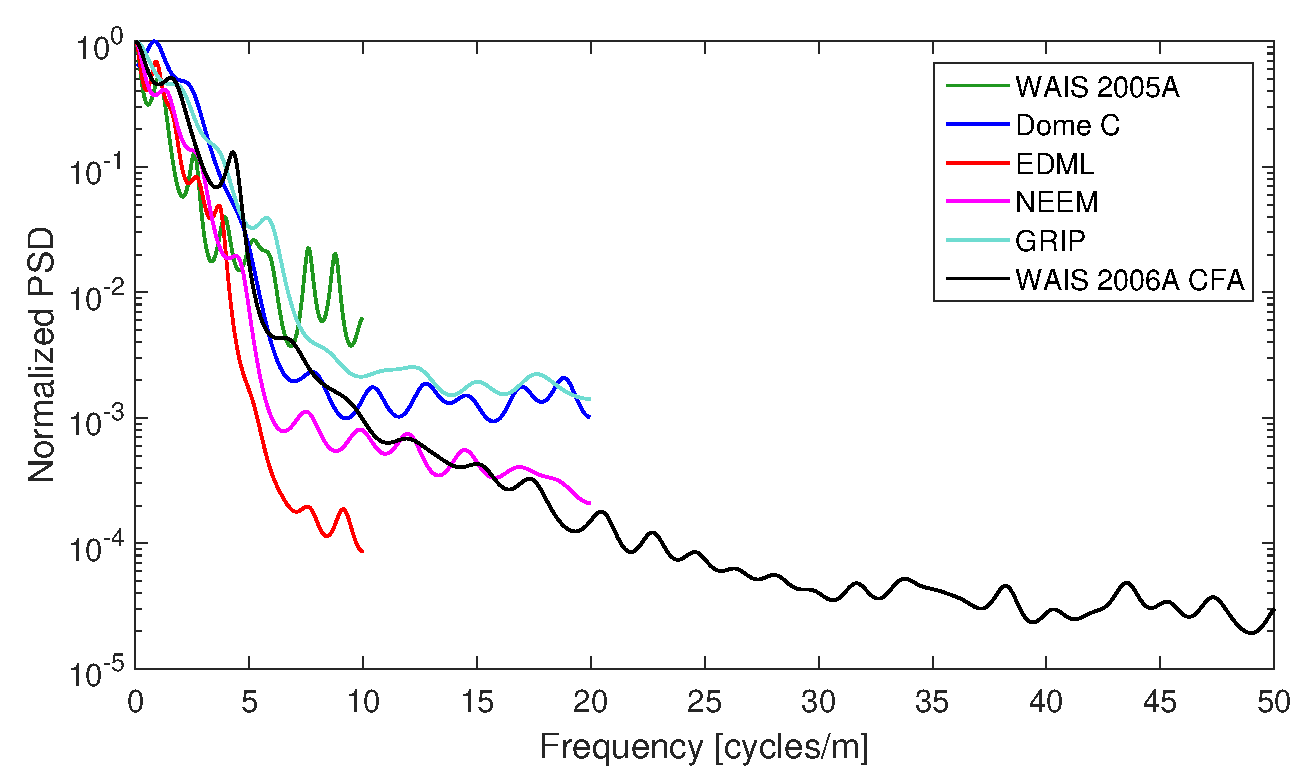
\includegraphics[width=0.9\linewidth]{PSD_discrete_plus_cfa_v1.eps}

	\end{minipage}%
	\begin{minipage}{0.5\textwidth}
		\centering
		\indent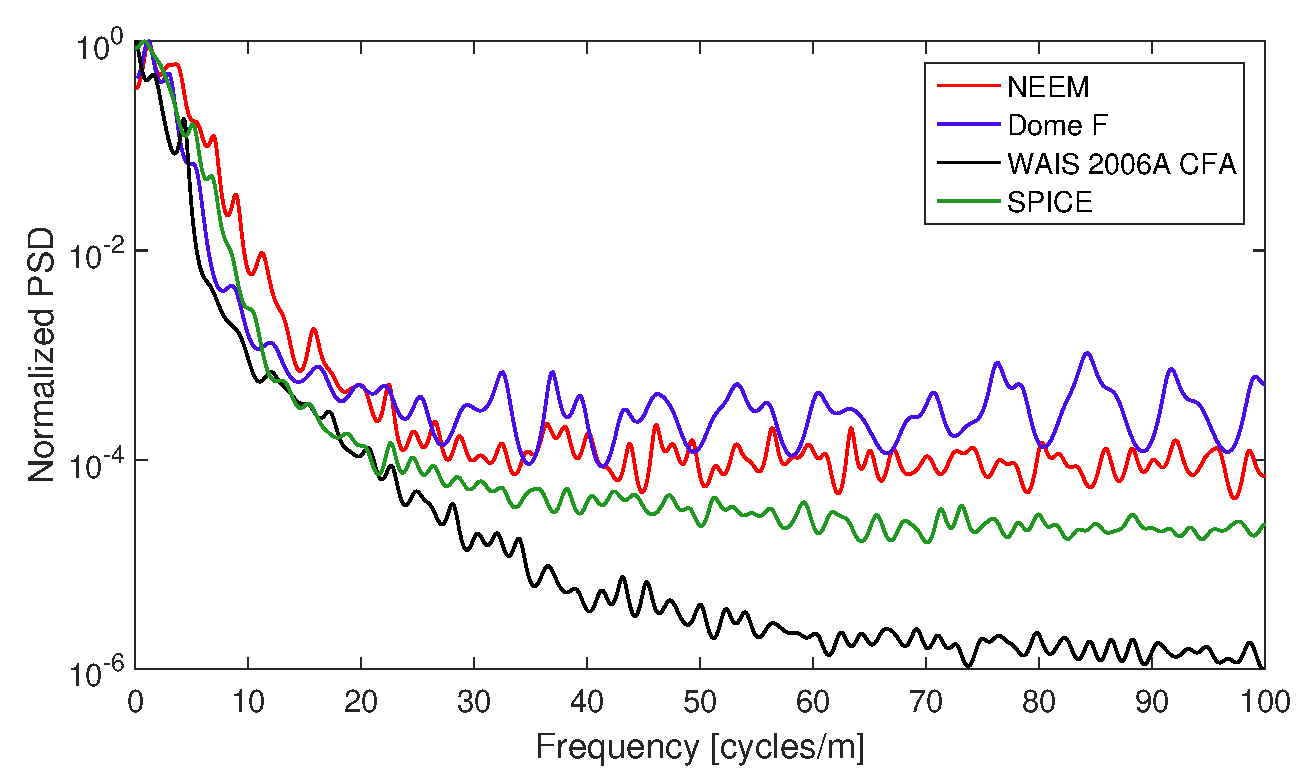
\includegraphics[width=0.9\linewidth]{PSD_CFA_v1.eps}

	\end{minipage}
	\caption{Left figure: The normalized PSD of five discretely measured $\delta^{18}$O series plotted together with the PSD of a $\delta^{18}$O WDC section. Right figure: The normalized PSD of four continuously measured $\delta$D series.}
\label{spectra_disVScfa}
\end{figure}

\begin{figure}
	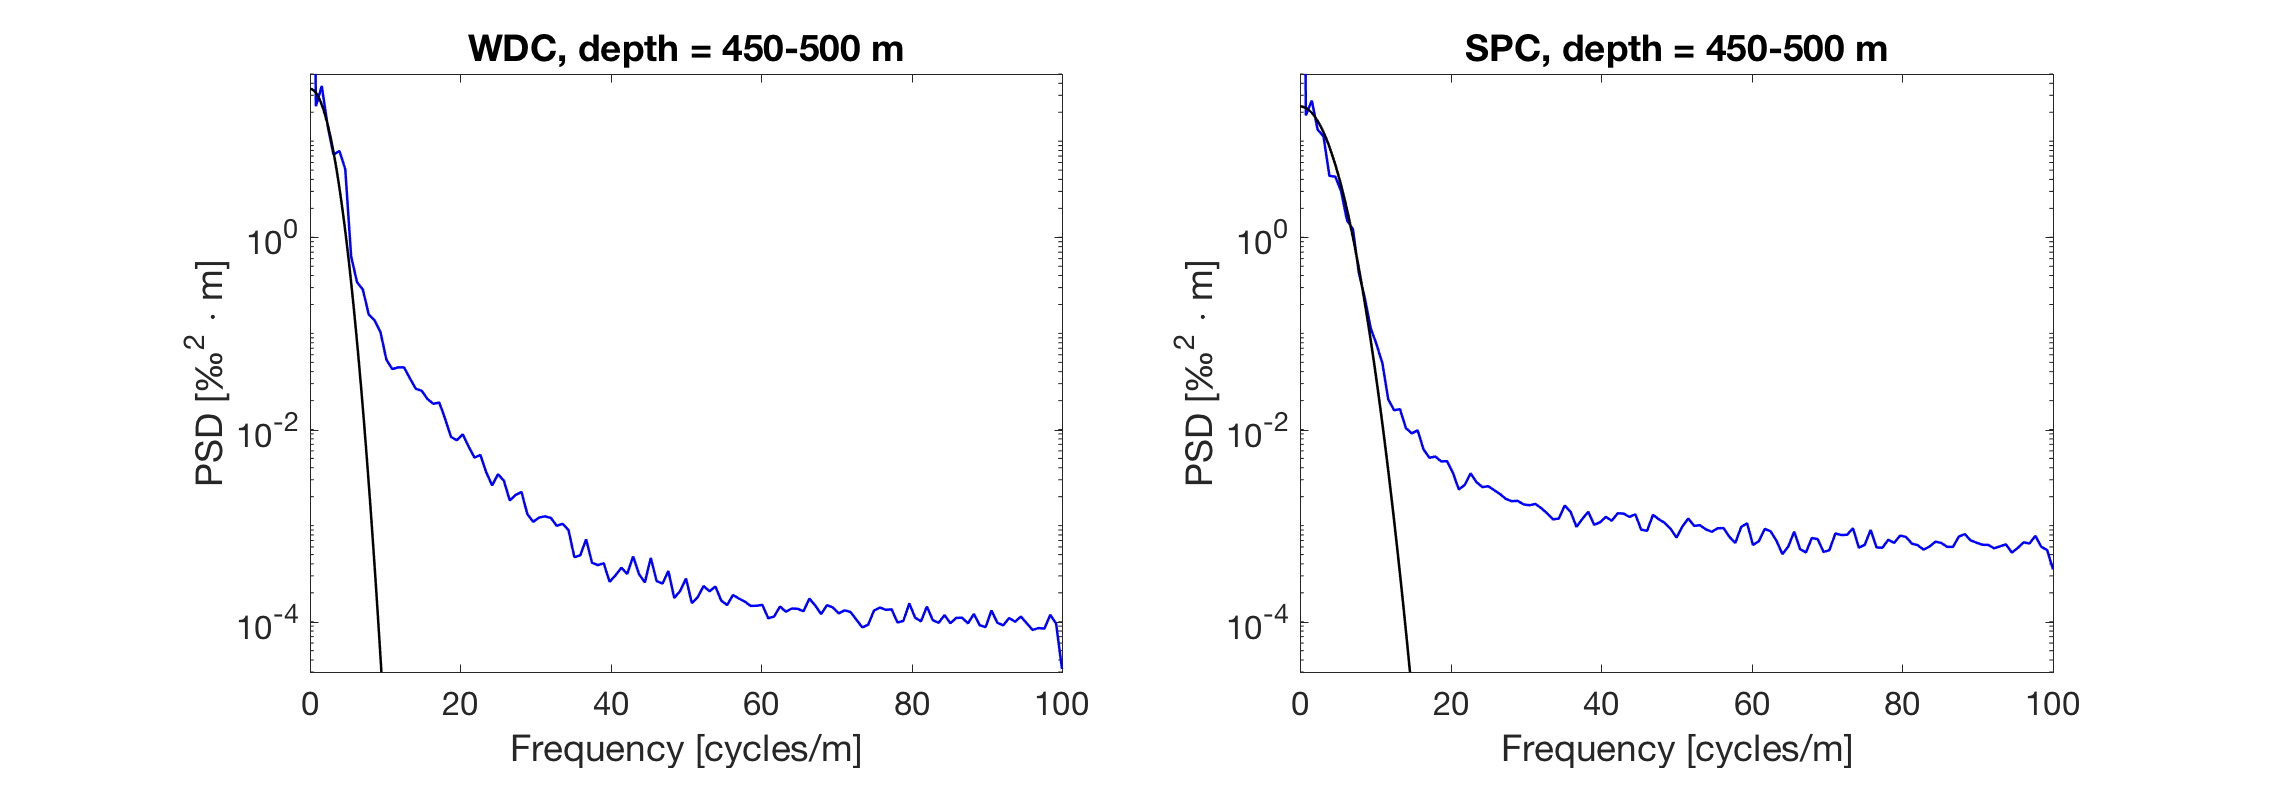
\includegraphics[width=\linewidth]{cutoff.eps}
	\caption{Cut-off technique on WDC and SPC at 450-500m depth. Blue curve is data spectrum and black curve is Gaussian fit.} \label{cutoff}
\end{figure}

\begin{figure}
	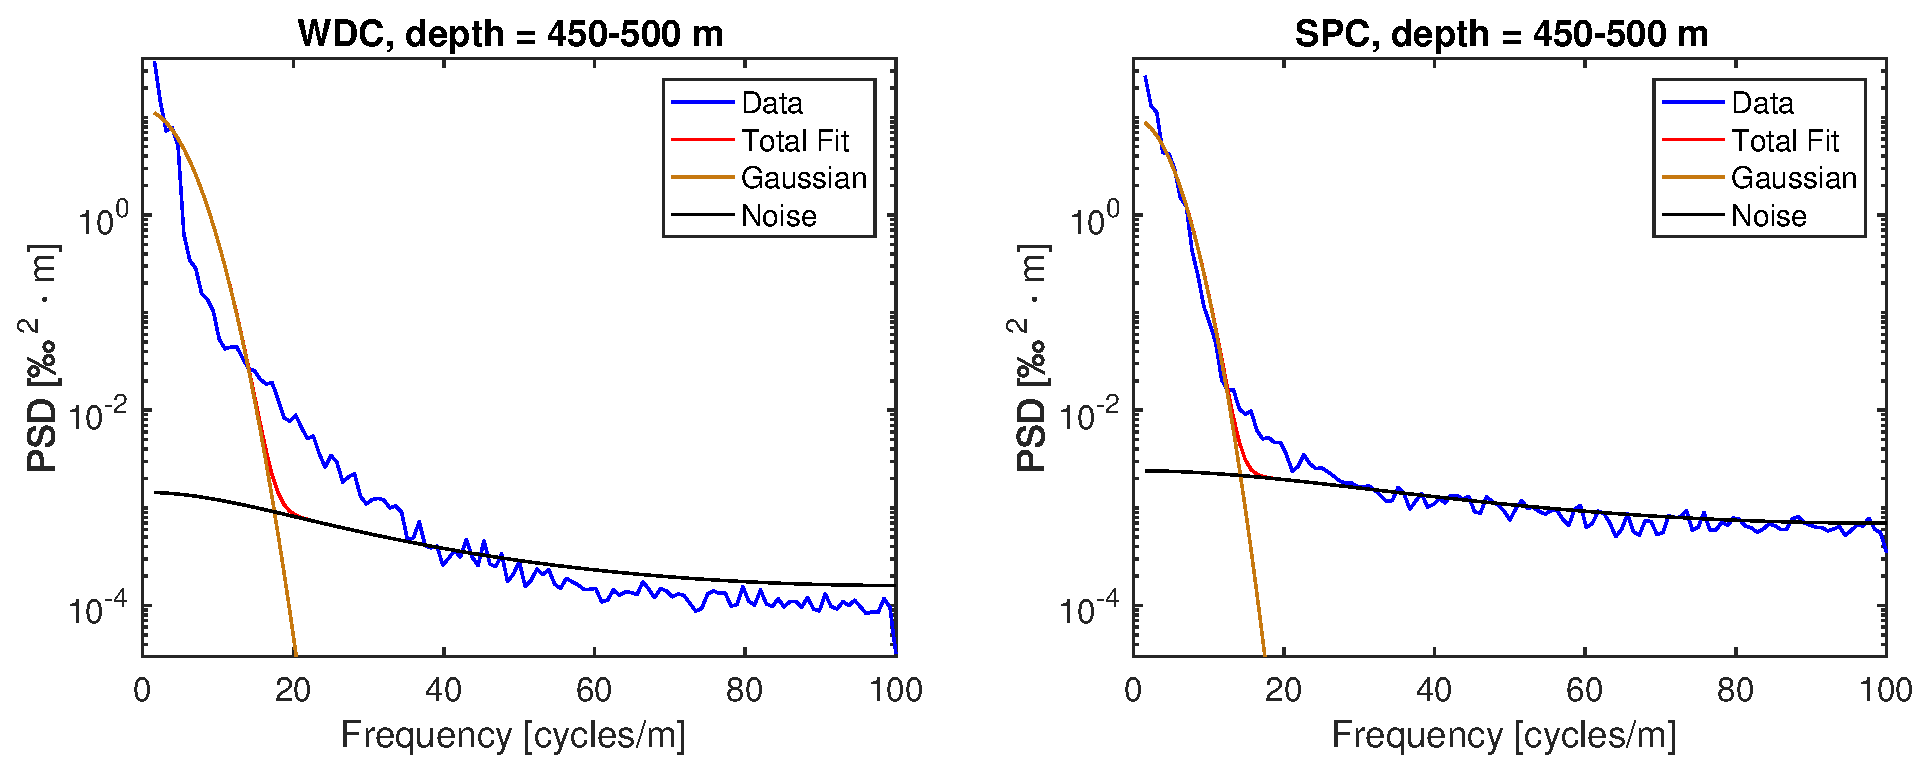
\includegraphics[width=\linewidth]{GR_fits.eps}
	\caption{Single-Gaussian multi-function fits for WDC and SPC at 450-500m depth.} \label{GR_fits}
\end{figure}

\begin{figure}
	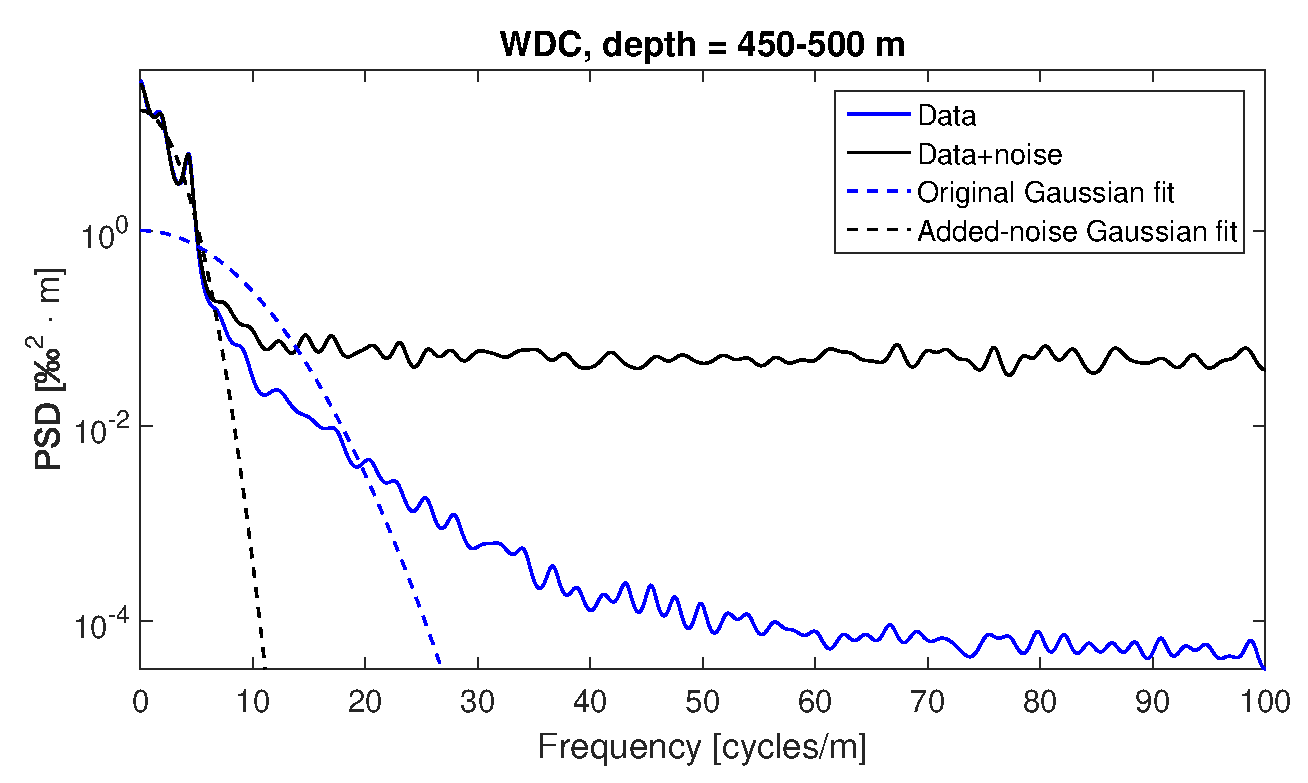
\includegraphics[width=.9\linewidth]{WAIS_spectrum_added_noise.eps}
	\caption{An illustration of the noise-adding technique for a $\delta$D section from WDC. The solid blue curve is the un-modified data and the black curve is data with noise added. The dashed lines represent the Gaussian functions fit using the two-function fitting technique.} \label{WAIS_spectrum_added_noise}
\end{figure}

\begin{figure}
	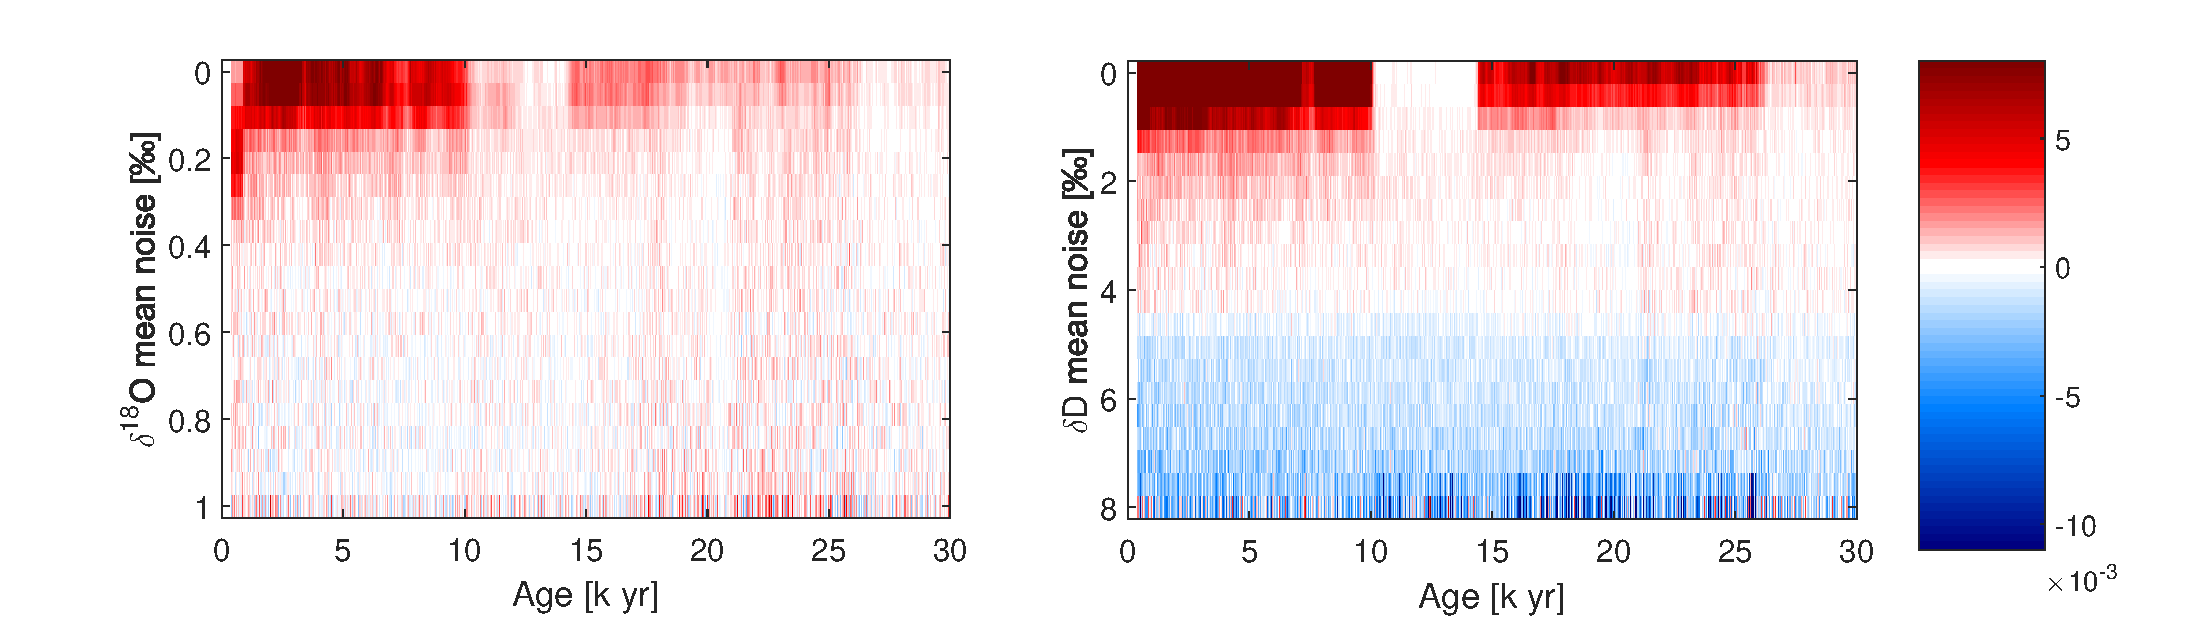
\includegraphics[width=\linewidth]{added_noise_sensitivity.eps}
	\caption{For WDC, the gradient of estimated diffusion lengths with respect to noise level plotted as a function of age. At each age, the lowest noise-level with a gradient of approximately zero is chosen as the optimal noise-level to be added.} \label{added_noise_sensitivity}
\end{figure}

\begin{figure}
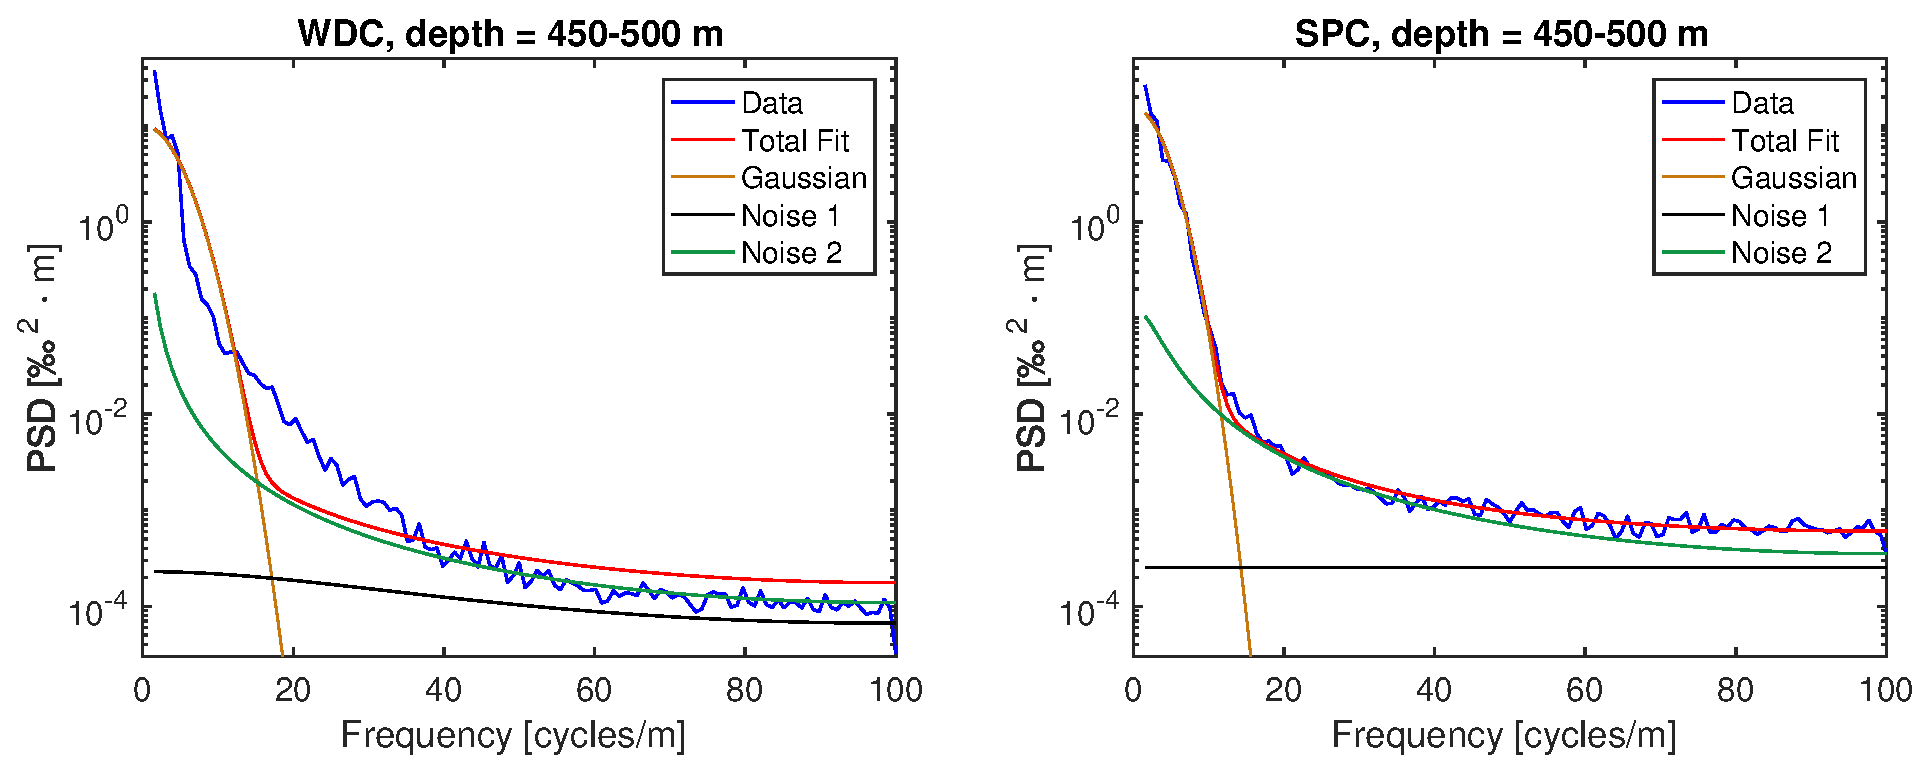
\includegraphics[width=.9\linewidth]{GRR_fits.eps}
\caption{Single Gaussian and two autoregressive-noise functions fit to WDC and SPC spectra.}\label{GRR_fits}
\end{figure}

\begin{figure}
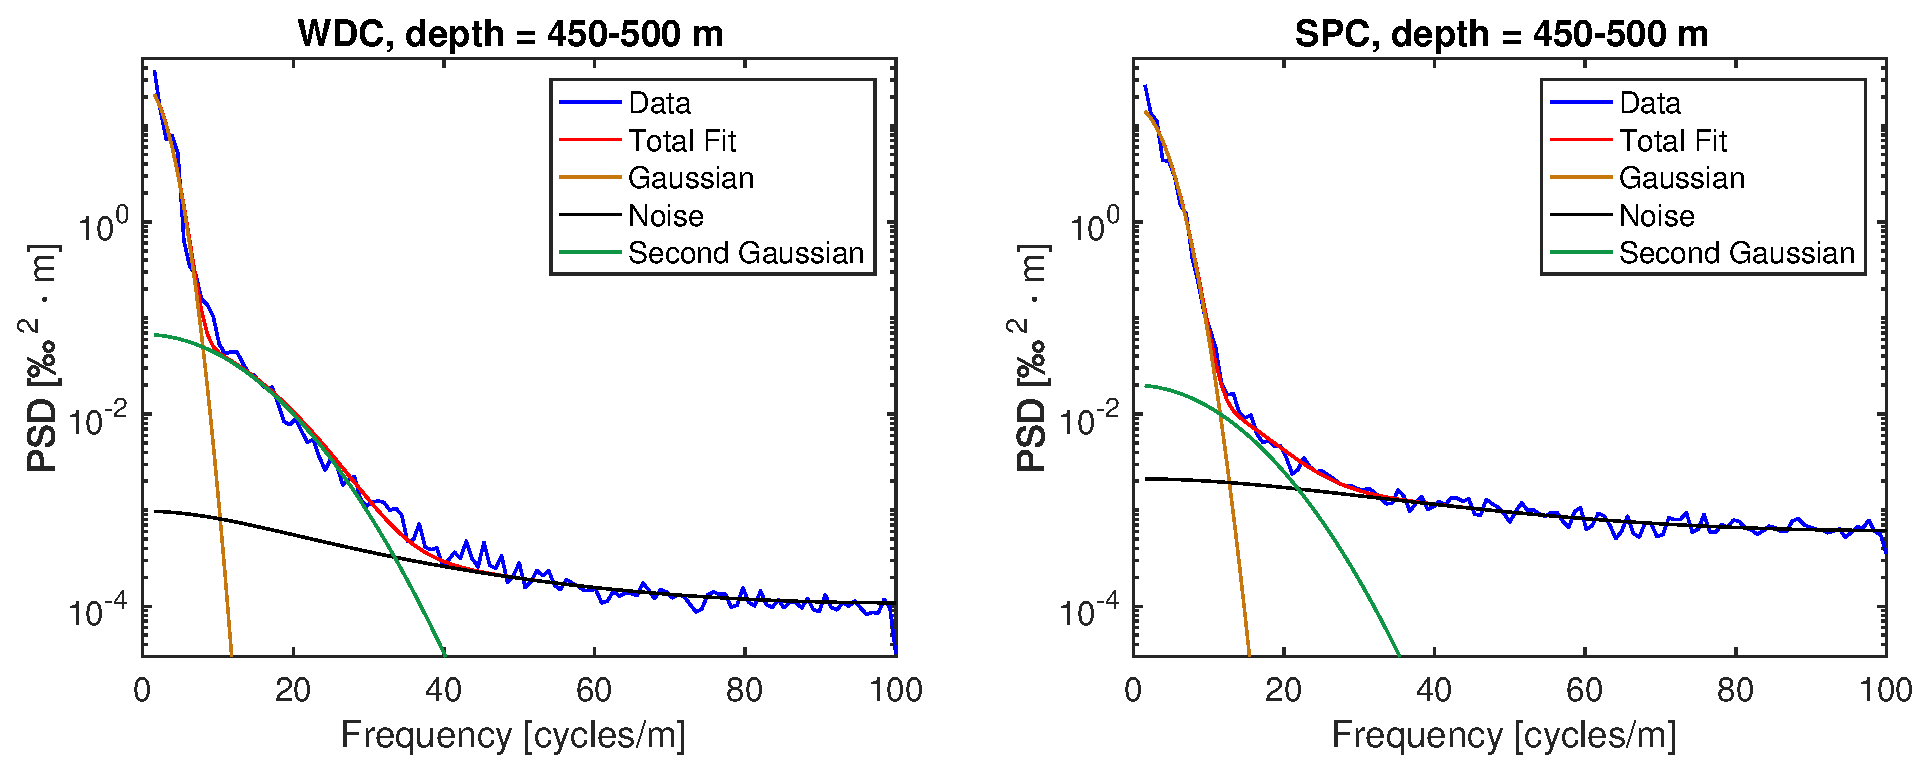
\includegraphics[width=.9\linewidth]{GGR_fits.eps}
\caption{Double-Gaussian multi-function technique fit to WDC and SPC spectra.}\label{GGR_fits}
\end{figure}

\begin{figure}
	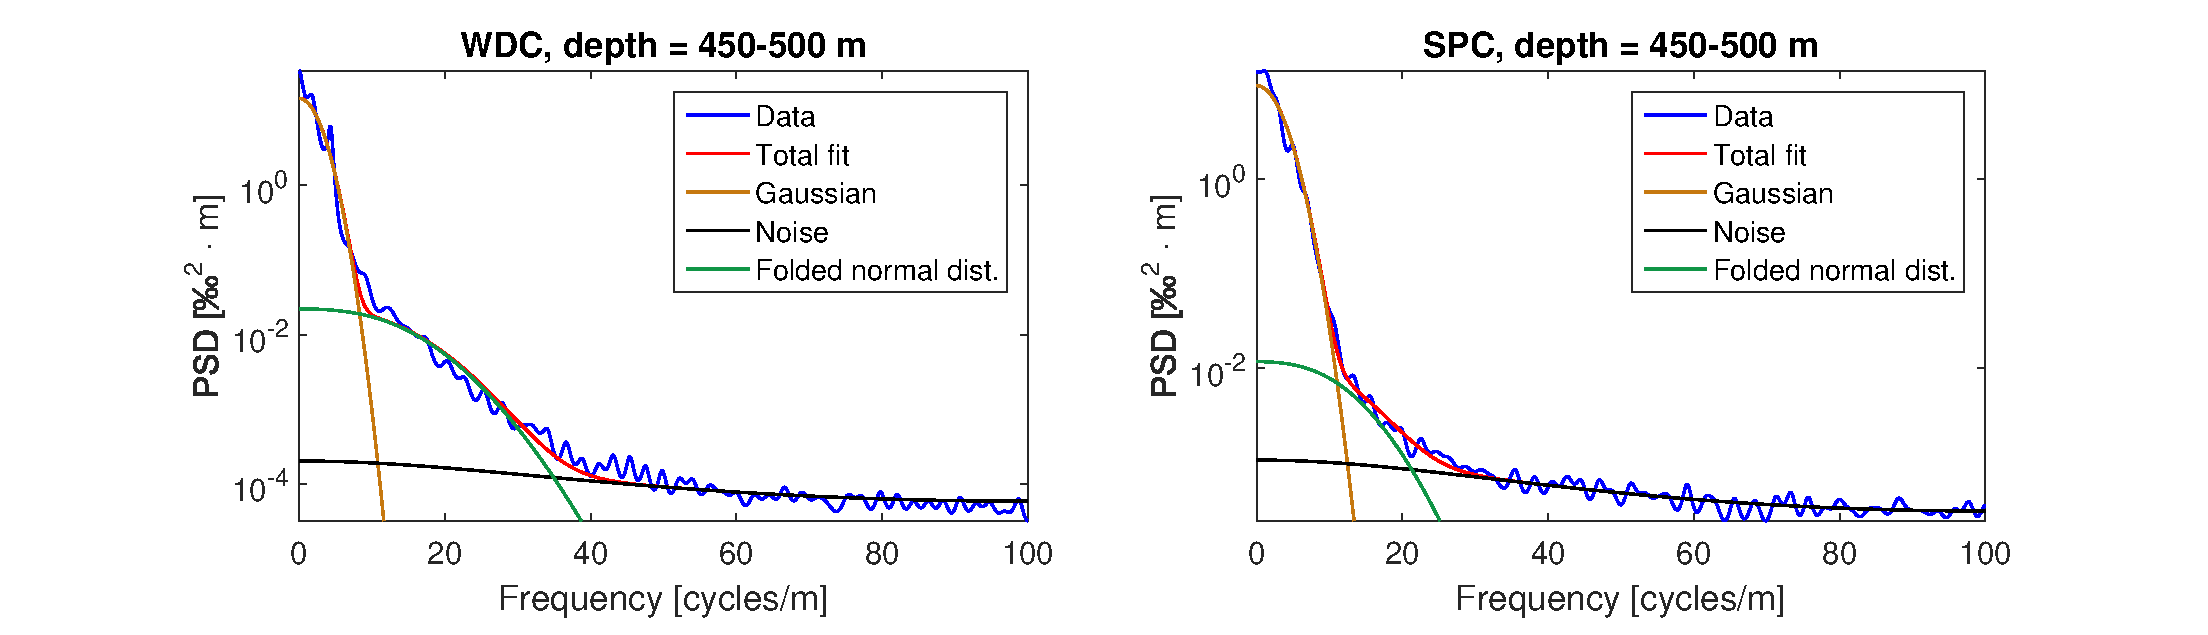
\includegraphics[width=1.1\linewidth]{folded_normal_gauss_spectrum.eps}
	\caption{Folded normal distribution multi-function technique fit to WDC and SPC spectra.}\label{folded_normal_gauss_spectrum}
\end{figure}

\begin{figure}
	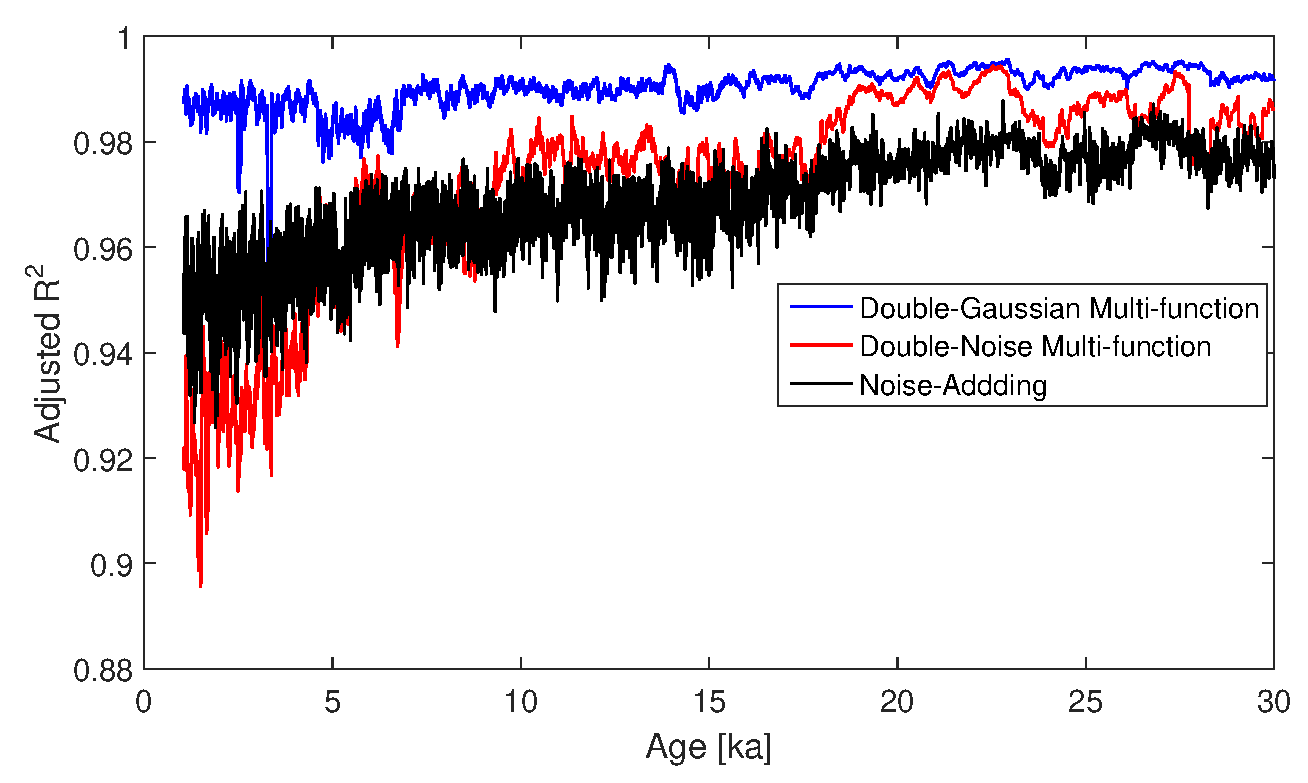
\includegraphics[width=.9\linewidth]{G_of_fit_1.eps}
	\caption{For WDC, the adjusted goodness of fit calculations through age for each fitting technique. FND results are identical to the results of a Gaussian curve and are not shown.} \label{G_of_fit_1}
\end{figure}

\begin{figure}
	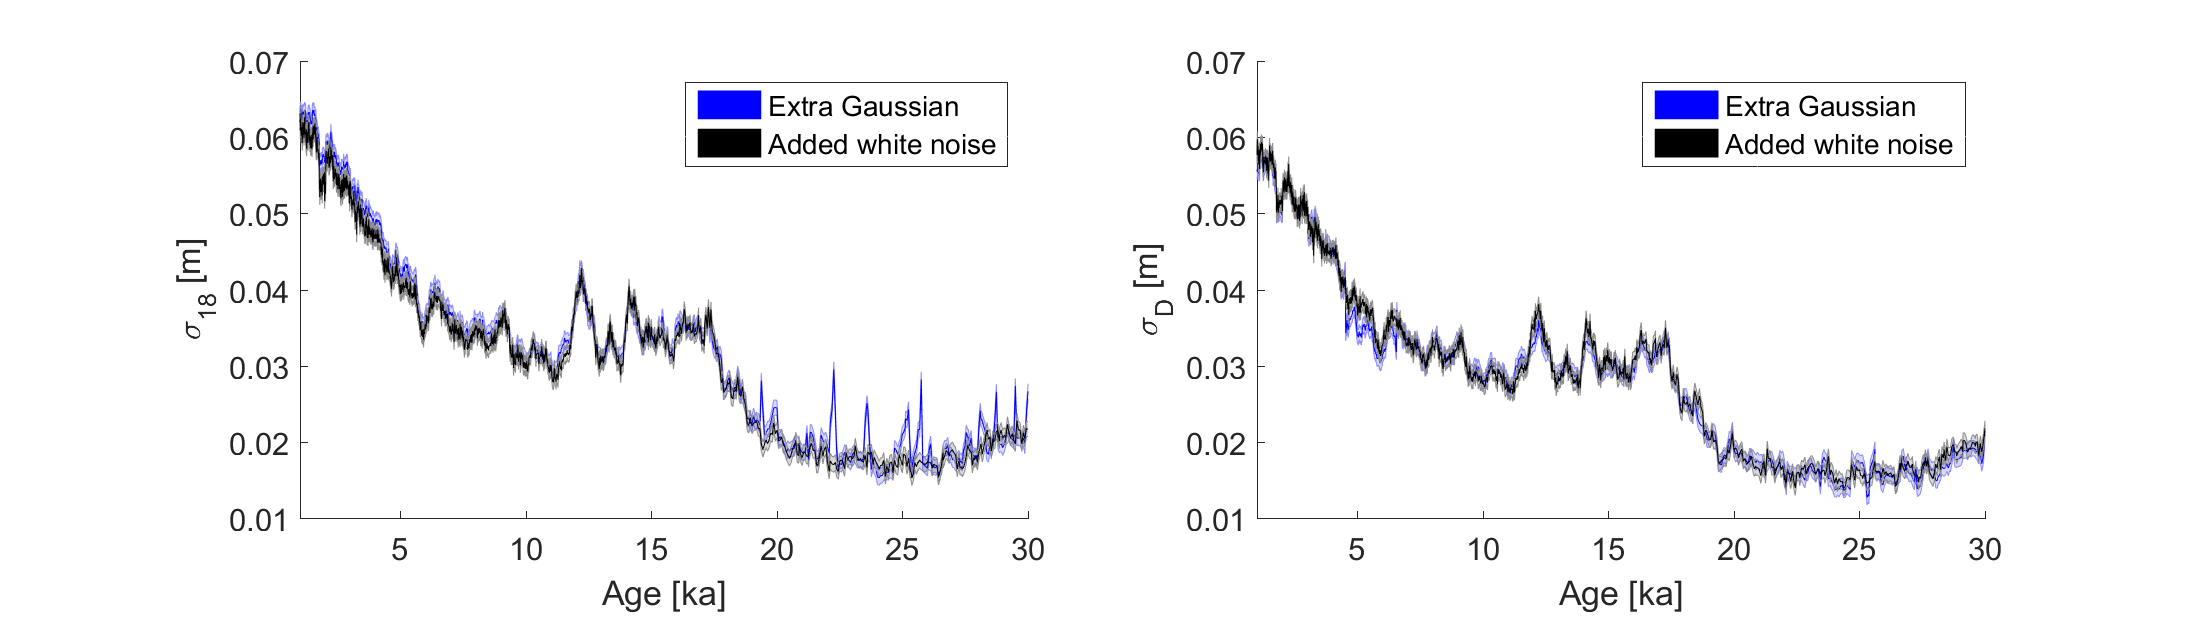
\includegraphics[width=\linewidth]{WAIS_diffusion_adding_noise.eps}
	\caption{WDC diffusion lengths of $\delta^{18}$O (left) and $\delta$D (right). Blue curve shows the multi-function Double-Gaussian technique, and the black curve shows the noise-adding technique.} \label{WAIS_diffusion_adding_noise}
\end{figure}

\begin{figure}
	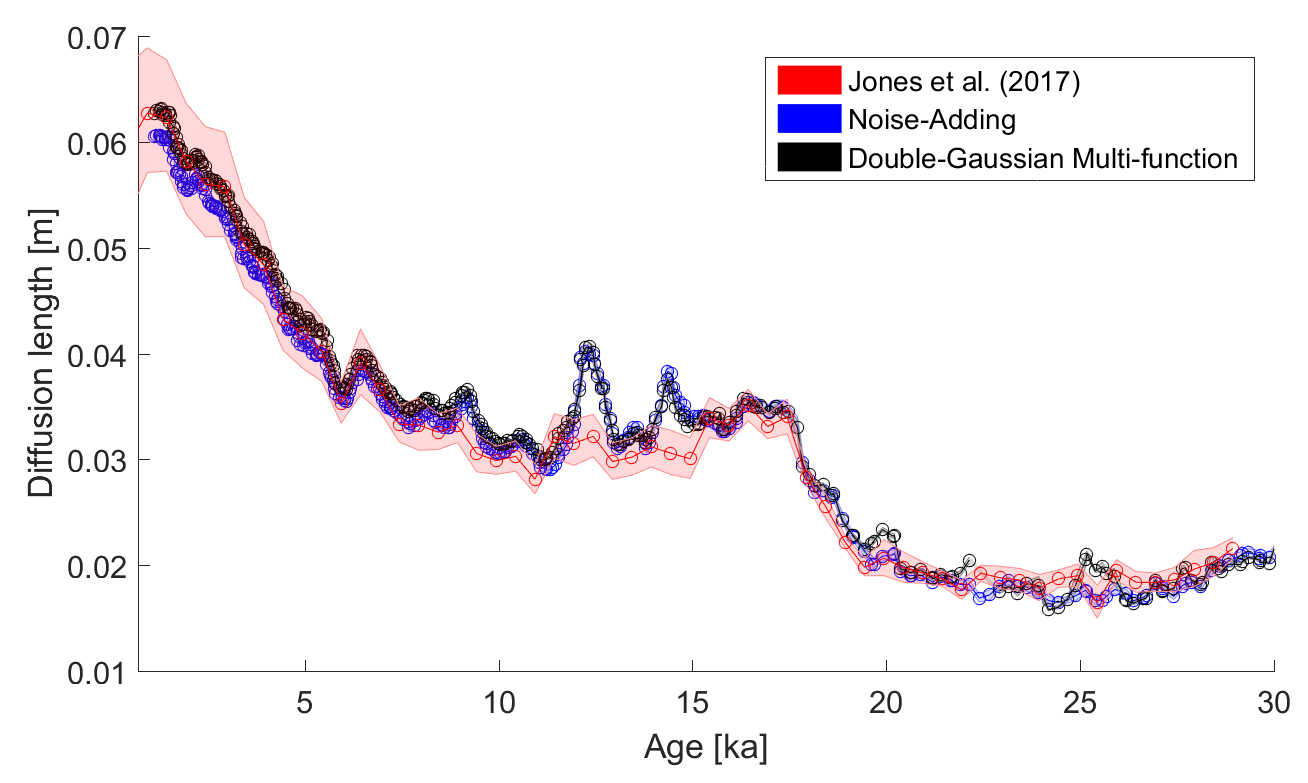
\includegraphics[width=.9\linewidth]{WAIS_diffusion_lengths.eps}
	\caption{Estimated WDC diffusion lengths of $\delta$D compared with those from \cite{Jones2017a}.} \label{WAIS_diffusion_lengths}
\end{figure}

\begin{figure}
	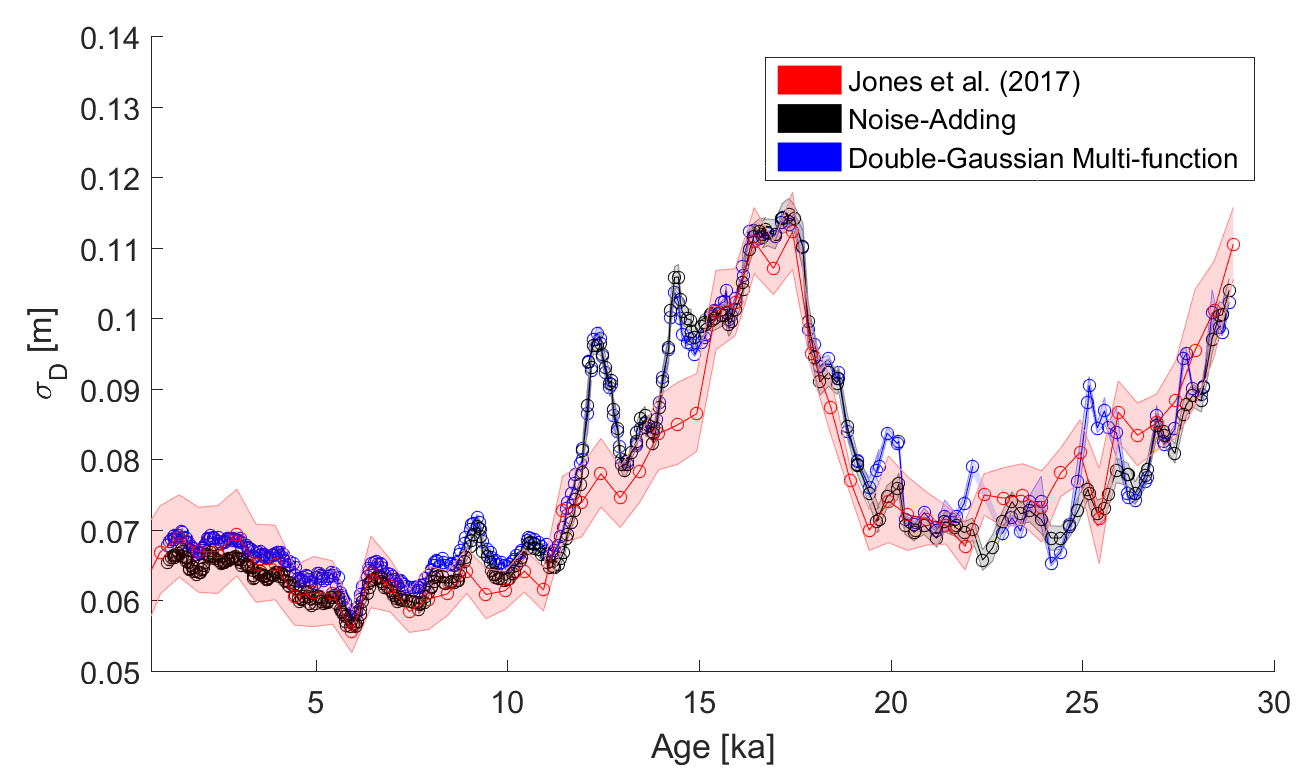
\includegraphics[width=.9\linewidth]{WAIS_diffusion_lengths_thinning_corr.eps}
	\caption{Thinning-corrected WDC diffusion lengths of $\delta$D  compared with those from \cite{Jones2017a}.} \label{WAIS_diffusion_lengths_thinning_corr}
\end{figure}

\begin{table}
\caption{Temperature Estimates for SPC for 50-meter windows from 6.7 - 7.5 ka (450-500 meters) and 30.9-33.1 ka (1300 - 1350 meters). For each window, the noise-adding and double-Gaussian multi-function fitting techniques are used on on all available isotope data. The temperature difference between the two windows is also calculated. The means and standard deviations are given for each window, showing how well the techniques compare. All temperatures are in degrees C.}\label{SP_deltaT}
\begin{tabular}{c|c c|c c c|c c}
\textbf{Technique} & \multicolumn{2}{|c|}{\textbf{6.7 - 7.5 ka}} & \multicolumn{3}{|c|}{\textbf{30.9 - 33.1 ka}} & \multicolumn{2}{|c}{\textbf{Temperature Difference}}\\
 & \textbf{$\delta$D} & \textbf{$\delta^{18}$O} & \textbf{$\delta$D} & \textbf{$\delta^{18}$O} & \textbf{$\delta^{17}$O} & \textbf{$\Delta$T $\delta$D} & \textbf{$\Delta$T $\delta^{18}$O}\\
\hline
Noise-adding & -56.7 & -54.3 & -61.8 & -58.4 & -56.8 & 5.1 & 4.1 \\
Double-Gaussian & -55.6 & -53.5 & -58.9 & -57.6 & -57.3 & 3.3 & 4.2 \\
\hline
mean & \multicolumn{2}{|c|}{-55.0} & \multicolumn{3}{|c|}{-58.5} & \multicolumn{2}{|c}{4.2} \\
standard deviation & \multicolumn{2}{|c|}{1.4} & \multicolumn{3}{|c|}{1.8} & \multicolumn{2}{|c}{0.7} \\
\end{tabular}
\end{table}

\end{document}

%%%%%%%%%%%%%%%%%%%%%%%%%%%%%%%%%%%%%%%%%%%%%%%%%%%%%%%%%%%%%%%

More Information and Advice:

%% ------------------------------------------------------------------------ %%
%
%  SECTION HEADS
%
%% ------------------------------------------------------------------------ %%

% Capitalize the first letter of each word (except for
% prepositions, conjunctions, and articles that are
% three or fewer letters).

% AGU follows standard outline style; therefore, there cannot be a section 1 without
% a section 2, or a section 2.3.1 without a section 2.3.2.
% Please make sure your section numbers are balanced.
% ---------------
% Level 1 head
%
% Use the \section{} command to identify level 1 heads;
% type the appropriate head wording between the curly
% brackets, as shown below.
%
%An example:
%\section{Level 1 Head: Introduction}
%
% ---------------
% Level 2 head
%
% Use the \subsection{} command to identify level 2 heads.
%An example:
%\subsection{Level 2 Head}
%
% ---------------
% Level 3 head
%
% Use the \subsubsection{} command to identify level 3 heads
%An example:
%\subsubsection{Level 3 Head}
%
%---------------
% Level 4 head
%
% Use the \subsubsubsection{} command to identify level 3 heads
% An example:
%\subsubsubsection{Level 4 Head} An example.
%
%% ------------------------------------------------------------------------ %%
%
%  IN-TEXT LISTS
%
%% ------------------------------------------------------------------------ %%
%
% Do not use bulleted lists; enumerated lists are okay.
% \begin{enumerate}
% \item
% \item
% \item
% \end{enumerate}
%
%% ------------------------------------------------------------------------ %%
%
%  EQUATIONS
%
%% ------------------------------------------------------------------------ %%

% Single-line equations are centered.
% Equation arrays will appear left-aligned.

Math coded inside display math mode \[ ...\]
 will not be numbered, e.g.,:
 \[ x^2=y^2 + z^2\]

 Math coded inside \begin{equation} and \end{equation} will
 be automatically numbered, e.g.,:
 \begin{equation}
 x^2=y^2 + z^2
 \end{equation}

% IF YOU HAVE MULTI-LINE EQUATIONS, PLEASE
% BREAK THE EQUATIONS INTO TWO OR MORE LINES
% OF SINGLE COLUMN WIDTH (20 pc, 8.3 cm)
% using double backslashes (\\).

% To create multiline equations, use the
% \begin{eqnarray} and \end{eqnarray} environment
% as demonstrated below.
\begin{eqnarray}
  x_{1} & = & (x - x_{0}) \cos \Theta \nonumber \\
        && + (y - y_{0}) \sin \Theta  \nonumber \\
  y_{1} & = & -(x - x_{0}) \sin \Theta \nonumber \\
        && + (y - y_{0}) \cos \Theta.
\end{eqnarray}

%If you don't want an equation number, use the star form:
%\begin{eqnarray*}...\end{eqnarray*}

% Break each line at a sign of operation
% (+, -, etc.) if possible, with the sign of operation
% on the new line.

% Indent second and subsequent lines to align with the first character following the equal sign on the first line.

% Use an \hspace{} command to insert horizontal space into your equation if necessary. Place an appropriate unit of measure between the curly braces, e.g. \hspace{1in}; you may have to experiment to achieve the correct amount of space.


%% ------------------------------------------------------------------------ %%
%
%  EQUATION NUMBERING: COUNTER
%
%% ------------------------------------------------------------------------ %%

% You may change equation numbering by resetting
% the equation counter or by explicitly numbering
% an equation.

% To explicitly number an equation, type \eqnum{}
% (with the desired number between the brackets)
% after the \begin{equation} or \begin{eqnarray}
% command.  The \eqnum{} command will affect only
% the equation it appears with; LaTeX will number
% any equations appearing later in the manuscript
% according to the equation counter.
%

% If you have a multiline equation that needs only
% one equation number, use a \nonumber command in
% front of the double backslashes (\\) as shown in
% the multiline equation above.

%% ------------------------------------------------------------------------ %%
%
%  SIDEWAYS FIGURE AND TABLE EXAMPLES
%
%% ------------------------------------------------------------------------ %%
%
% For tables and figures, add \usepackage{rotating} to the paper and add the rotating.sty file to the folder.
% AGU prefers the use of {sidewaystable} over {landscapetable} as it causes fewer problems.
%
% \begin{sidewaysfigure}
% \includegraphics[width=20pc]{samplefigure.eps}
% \caption{caption here}
% \label{label_here}
% \end{sidewaysfigure}
%
% \begin{sidewaystable}
% \caption{}
% \begin{tabular}
% Table layout here.
% \end{tabular}
% \end{sidewaystable}
